%% ============================================================
%%  RAPPORT PFA — TAQA IT SMART HELPDESK
%%  ENSIASD Taroudant — Université Ibn Zohr
%%  Auteur  : Mohammed REGRAGUI
%%  Version : 1.0 — Septembre 2025
%%  Compilez avec : pdflatex -> pdflatex -> pdflatex
%%  (Si bibliographie : pdflatex -> bibtex -> pdflatex x2)
%%
%%  NOTE : Placez ce fichier dans le dossier contenant :
%%    - report_figures/ (fig_architecture.png, fig_usecase.png, etc.)
%%    - frontend/src/assets/logo_taqa.png
%% ============================================================

\documentclass[12pt, a4paper, oneside]{report}

%% ─── ENCODAGE & LANGUE ──────────────────────────────────────
\usepackage[T1]{fontenc}
\usepackage[utf8]{inputenc}
\usepackage[french]{babel}
\usepackage{lmodern}
\usepackage{microtype}

%% ─── MISE EN PAGE ───────────────────────────────────────────
\usepackage[
  top=2.5cm, bottom=2.5cm,
  left=3cm,  right=2.5cm,
  headheight=15pt
]{geometry}
\usepackage{setspace}
\onehalfspacing
\usepackage{emptypage}
\usepackage{parskip}
\setlength{\parindent}{0pt}
\setlength{\parskip}{6pt}

%% ─── POLICE ─────────────────────────────────────────────────
\usepackage[scaled=0.92]{helvet}
\renewcommand{\familydefault}{\sfdefault}

%% ─── COULEURS TAQA MOROCCO ──────────────────────────────────
\usepackage[dvipsnames,table]{xcolor}
\definecolor{taqaNavy}{RGB}{10,  24,  64}
\definecolor{taqaCyan}{RGB}{0,  174, 239}
\definecolor{taqaBlue}{RGB}{0,   82, 165}
\definecolor{taqaGold}{RGB}{234, 170,   0}
\definecolor{taqaGray}{RGB}{100, 110, 130}
\definecolor{taqaLight}{RGB}{240, 245, 255}
\definecolor{codebg}{RGB}{245, 247, 252}
\definecolor{coderule}{RGB}{200, 215, 240}

%% ─── GRAPHIQUES ─────────────────────────────────────────────
\usepackage{graphicx}
\usepackage{float}
\graphicspath{{report_figures/}}

%% ─── TABLEAUX ───────────────────────────────────────────────
\usepackage{booktabs}
\usepackage{tabularx}
\usepackage{multirow}
\usepackage{longtable}
\usepackage{array}
\renewcommand{\arraystretch}{1.35}

%% ─── CODE SOURCE ────────────────────────────────────────────
\usepackage{listings}
\lstset{
  backgroundcolor=\color{codebg},
  basicstyle=\ttfamily\footnotesize,
  breaklines=true,
  breakatwhitespace=true,
  captionpos=b,
  commentstyle=\color{taqaGray}\itshape,
  frame=single,
  framesep=5pt,
  framerule=0.6pt,
  rulecolor=\color{coderule},
  keywordstyle=\color{taqaBlue}\bfseries,
  stringstyle=\color{taqaCyan},
  numbers=left,
  numberstyle=\tiny\color{taqaGray},
  numbersep=8pt,
  showstringspaces=false,
  tabsize=4,
  xleftmargin=15pt,
  xrightmargin=5pt,
  aboveskip=10pt,
  belowskip=10pt,
}
\lstdefinestyle{python}{
  language=Python,
  morekeywords={def,return,import,from,as,class,try,except,with,
                None,True,False,self,predict,transform,joblib,load},
}
\lstdefinestyle{bash}{
  language=bash,
  morekeywords={cd,npm,python,pip,ollama,echo,start,timeout},
}

%% ─── EN-TÊTES & PIEDS DE PAGE ───────────────────────────────
\usepackage{fancyhdr}
\pagestyle{fancy}
\fancyhf{}
\fancyhead[L]{\textcolor{taqaGray}{\footnotesize\textit{TAQA IT Smart Helpdesk — Rapport PFA}}}
\fancyhead[R]{\textcolor{taqaGray}{\footnotesize\textit{ENSIASD Taroudant — 2024/2025}}}
\fancyfoot[C]{\textcolor{taqaGray}{\footnotesize---~\thepage~---}}
\renewcommand{\headrulewidth}{0.4pt}
\renewcommand{\headrule}{\hbox to\headwidth{\color{taqaCyan}\leaders\hrule height \headrulewidth\hfill}}

%% ─── CHAPITRES & SECTIONS ───────────────────────────────────
\usepackage{titlesec}
\titleformat{\chapter}[display]
  {\normalfont\huge\bfseries\color{taqaNavy}}
  {\color{taqaCyan}\rule{\textwidth}{2pt}\\[6pt]%
   \hfill{\normalfont\large\color{taqaGray}\MakeUppercase{Chapitre}~\thechapter}}
  {10pt}
  {\Huge\color{taqaNavy}}
  [\vspace{4pt}\color{taqaCyan}\rule{\textwidth}{1pt}\vspace{10pt}]

\titleformat{\section}
  {\normalfont\Large\bfseries\color{taqaBlue}}{\thesection.}{0.5em}{}
\titleformat{\subsection}
  {\normalfont\large\bfseries\color{taqaNavy}}{\thesubsection.}{0.5em}{}
\titleformat{\subsubsection}
  {\normalfont\normalsize\bfseries\color{taqaGray}}{\thesubsubsection.}{0.4em}{}
\titlespacing*{\chapter}{0pt}{-20pt}{30pt}

%% ─── LIENS PDF ──────────────────────────────────────────────
\usepackage[
  pdftitle={Rapport PFA — TAQA IT Smart Helpdesk},
  pdfauthor={Mohammed REGRAGUI},
  pdfsubject={Plateforme ITSM Intelligente NLP, ML et LLM},
  colorlinks=true,
  linkcolor=taqaBlue,
  citecolor=taqaNavy,
  urlcolor=taqaCyan,
  bookmarks=true,
]{hyperref}

%% ─── BOÎTES TCOLORBOX ───────────────────────────────────────
\usepackage[most]{tcolorbox}
\tcbuselibrary{breakable,skins,listings}

\newtcolorbox{remarque}[1][]{
  enhanced, breakable,
  colback=taqaLight, colframe=taqaCyan,
  fonttitle=\bfseries\color{taqaNavy},
  title={Remarque},
  left=6pt, right=6pt, top=4pt, bottom=4pt,
  borderline west={3pt}{0pt}{taqaCyan},
  boxrule=0.5pt, #1
}

\newtcolorbox{resultat}[1][]{
  enhanced, breakable,
  colback={taqaNavy!6}, colframe=taqaNavy,
  fonttitle=\bfseries\color{white}, coltitle=white,
  attach boxed title to top left={yshift=-2mm, xshift=5mm},
  boxed title style={colback=taqaNavy, colframe=taqaNavy, sharp corners},
  title={Resultat cle},
  left=8pt, right=8pt, top=8pt, bottom=6pt,
  boxrule=0.8pt, #1
}

%% ─── MATHS ──────────────────────────────────────────────────
\usepackage{amsmath,amssymb}

%% ─── NUMÉROTATION ───────────────────────────────────────────
\usepackage{chngcntr}
\counterwithin{figure}{chapter}
\counterwithin{table}{chapter}

%% ─── TABLE DES MATIÈRES ─────────────────────────────────────
\usepackage{tocloft}
\setlength{\cftbeforechapskip}{6pt}
\renewcommand{\cftchapfont}{\bfseries\color{taqaNavy}}
\renewcommand{\cftchappagefont}{\bfseries\color{taqaNavy}}

%% ─── DIVERS ─────────────────────────────────────────────────
\usepackage{enumitem}
\setlist[itemize]{leftmargin=*, label=\textcolor{taqaCyan}{$\triangleright$}}
\setlist[enumerate]{leftmargin=*, label=\textcolor{taqaNavy}{\arabic*.}}
\usepackage{caption}
\captionsetup{
  font=small,
  labelfont={bf,color=taqaNavy},
  textfont={it,color=taqaGray},
  labelsep=period, skip=6pt,
}

%% ════════════════════════════════════════════════════════════
%%  DÉBUT DU DOCUMENT
%% ════════════════════════════════════════════════════════════
\begin{document}

%% ─── PAGE DE GARDE ──────────────────────────────────────────
\begin{titlepage}
\pagecolor{taqaNavy}
\color{white}
\begin{center}
  \vspace*{0.2cm}

  %% Bande institutionnelle
  \textcolor{taqaCyan}{\rule{\textwidth}{3pt}}
  \vspace{0.2cm}

  {\footnotesize\color{taqaCyan}
   \textbf{ROYAUME DU MAROC} \quad|\quad
   \textbf{UNIVERSITE IBN ZOHR — AGADIR}}\\[6pt]
  {\small\bfseries\color{taqaCyan}
   ECOLE NATIONALE SUPERIEURE DE L'INTELLIGENCE ARTIFICIELLE\\
   ET SCIENCES DES DONNEES (ENSIASD) — TAROUDANT}

  \vspace{0.5cm}
  \textcolor{taqaCyan}{\rule{0.5\textwidth}{0.8pt}}
  \vspace{0.3cm}

  %% Logo TAQA
  
\includegraphics[width=6cm,keepaspectratio]{logo_taqa}

  \vspace{0.5cm}
  {\large\bfseries RAPPORT DE PROJET DE FIN D'ANNEE (PFA)}\\[4pt]
  {\normalsize\color{taqaGold}\itshape
   Filiere : Sciences des Donnees, Big Data \& Intelligence Artificielle}

  \vspace{0.6cm}

  %% Titre principal
  \fcolorbox{taqaCyan}{taqaBlue!80!taqaNavy}{%
    \begin{minipage}{0.90\textwidth}
      \vspace{0.5cm}
      \centering
      {\Large\bfseries\color{white}
       CONCEPTION ET DEPLOIEMENT D'UNE\\[4pt]
       PLATEFORME ITSM INTELLIGENTE}\\[8pt]
      {\normalsize\color{taqaLight}
       Basee sur le NLP (spaCy), le Machine Learning Multi-Sorties\\
       et un Agent Conversationnel LLM (LLaMA~3.2 / RAG Deterministe)}\\[6pt]
      {\small\bfseries\color{taqaGold}
       Application au Support Technique de TAQA Morocco}
      \vspace{0.5cm}
    \end{minipage}%
  }

  \vspace{0.7cm}
  {\normalsize\color{taqaCyan}\textbf{TAQA IT Smart Helpdesk}
   — Centrale Thermique de Jorf Lasfar}

  \vspace{0.7cm}
  \textcolor{taqaCyan}{\rule{0.55\textwidth}{0.6pt}}
  \vspace{0.4cm}

  {\normalsize Presente par :}\\[5pt]
  {\Large\bfseries\color{taqaGold} Mohammed REGRAGUI}\\[3pt]
  {\small\color{taqaGray} Etudiant en Sciences des Donnees \& Intelligence Artificielle}

  \vspace{0.7cm}
  \begin{minipage}{0.88\textwidth}
    \centering
    \footnotesize
    \begin{tabular}{lll}
      \toprule
      \rowcolor{taqaBlue!80}
      \textbf{\color{white}Titre} &
      \textbf{\color{white}Affiliation} &
      \textbf{\color{white}Role dans le Jury} \\
      \midrule
      Pr. & ENSIASD de Taroudant & President du Jury \\
      Pr. & ENSIASD de Taroudant & Examinateur \\
      Pr. & ENSIASD de Taroudant & Examinateur \\
      Pr. & ENSIASD de Taroudant & Encadrant Pedagogique \\
      M./Mme. & TAQA Morocco & Encadrant Industriel \\
      \bottomrule
    \end{tabular}
  \end{minipage}

  \vfill
  \textcolor{taqaCyan}{\rule{\textwidth}{1pt}}\\[3pt]
  {\small Annee Universitaire 2024 -- 2025
   \quad\textbullet\quad Soutenu en Juin 2025}
\end{center}
\end{titlepage}
\nopagecolor

%% ─── PAGES PRÉLIMINAIRES ────────────────────────────────────
\frontmatter

%% DÉDICACES
\chapter*{Dedicaces}
\addcontentsline{toc}{chapter}{Dedicaces}

\begin{center}
  \vspace*{1cm}
  \colorbox{taqaLight}{%
    \begin{minipage}{0.88\textwidth}
      \vspace{0.6cm}\centering
      {\normalsize\itshape\color{taqaNavy}
      A mes chers parents, dont l'amour inconditionnel, les sacrifices
      constants et les prieres bienveillantes ont illumine mon parcours
      et m'ont donne la force de perseverer face a chaque defi.\\[0.5cm]
      A mes freres et soeurs, pour leur tendresse, leur encouragement
      indefectible et leur soutien precieux a chaque instant.\\[0.5cm]
      A l'ensemble de mes enseignants et encadrants de l'ENSIASD de
      Taroudant, qui ont su transmettre avec generosite leur rigueur
      scientifique et leur passion pour l'Intelligence Artificielle.\\[0.5cm]
      A tous mes amis et collegues de promotion, en souvenir des moments
      intenses de partage, d'entraide et de camaraderie.}
      \vspace{0.6cm}
    \end{minipage}%
  }
\end{center}

%% REMERCIEMENTS
\chapter*{Remerciements}
\addcontentsline{toc}{chapter}{Remerciements}

Au terme de ce projet de fin d'annee, j'exprime ma profonde gratitude et mes
sinceres remerciements a toutes les personnes qui ont contribue a
l'accomplissement de ce travail.

Je tiens tout d'abord a remercier chaleureusement la direction generale et
l'equipe informatique de \textbf{\textcolor{taqaNavy}{TAQA Morocco}} pour
m'avoir ouvert leurs portes au sein de la Centrale Thermique de Jorf Lasfar.

J'adresse mes remerciements les plus respectueux a mon \textbf{encadrant
professionnel} au sein de TAQA Morocco, pour son accueil, son encadrement
bienveillant et ses orientations techniques pointues.

Mes vifs remerciements vont egalement a mon \textbf{encadrant pedagogique} a
l'\textbf{ENSIASD de Taroudant}, pour sa disponibilite permanente et sa rigueur
methodologique.

Enfin, j'exprime ma reconnaissance aux honorables \textbf{membres du jury}
d'avoir accepte d'examiner et d'evaluer ce travail.

%% RÉSUMÉ
\chapter*{Resume}
\addcontentsline{toc}{chapter}{Resume / Abstract}

\begin{tcolorbox}[
  enhanced, breakable,
  colback=taqaLight, colframe=taqaNavy,
  title={\textbf{Resume — Francais}},
  fonttitle=\color{white},
  attach boxed title to top left={yshift=-2mm,xshift=5mm},
  boxed title style={colback=taqaNavy},
  boxrule=1pt, left=8pt, right=8pt, top=8pt, bottom=8pt
]
Dans un environnement industriel hautement strategique tel que celui de
\textbf{TAQA Morocco}, premier producteur prive d'electricite au Royaume
(fournissant pres de 40\,\% de la demande nationale), la disponibilite
permanente des infrastructures informatiques est primordiale. Face aux
limites des Help Desks traditionnels, ce projet presente la conception et
le deploiement d'une plateforme ITSM intelligente : \textbf{TAQA IT Smart Helpdesk}.

La solution repose sur trois piliers technologiques :
\begin{enumerate}
  \item \textbf{Pipeline NLP spaCy} : masquage automatique des informations
        personnelles (PII) et lemmatisation linguistique.
  \item \textbf{Modele ML supervise multi-sorties} : MultiOutputClassifier
        (LinearSVC + TF-IDF bigrammes) atteignant \textbf{98,52\,\%} de
        precision sur 2\,367 tickets reels.
  \item \textbf{Moteur RAG deterministe + LLaMA~3.2} : 162 procedures
        techniques certifiees, hebergement On-Premise souverain via Ollama.
\end{enumerate}

\textbf{Mots-cles :} ITSM, NLP, spaCy, Machine Learning, LinearSVC, TF-IDF,
RAG Deterministe, LLaMA 3.2, Ollama, React 18, Flask, TAQA Morocco.
\end{tcolorbox}

\vspace{0.6cm}

\begin{tcolorbox}[
  enhanced, breakable,
  colback=taqaNavy!5, colframe=taqaBlue,
  title={\textbf{Abstract — English}},
  fonttitle=\color{white},
  attach boxed title to top left={yshift=-2mm,xshift=5mm},
  boxed title style={colback=taqaBlue},
  boxrule=1pt, left=8pt, right=8pt, top=8pt, bottom=8pt
]
In a critical industrial energy environment such as \textbf{TAQA Morocco} ---
the Kingdom's leading private electricity producer (approx. 40\,\% of national
demand) --- continuous IT availability is paramount. This capstone project
introduces an AI-powered ITSM platform: \textbf{TAQA IT Smart Helpdesk}.

Built on three core layers: (1)~a spaCy NLP preprocessing pipeline with PII
masking; (2)~a multi-output ML classifier (LinearSVC / TF-IDF) achieving
\textbf{98.52\,\%} accuracy on 2,367 production tickets; (3)~a deterministic
RAG engine coupled with On-Premise LLaMA~3.2 and 162 certified solutions.

\textbf{Keywords:} ITSM, NLP, spaCy, Machine Learning, LinearSVC, TF-IDF,
Deterministic RAG, LLaMA 3.2, React 18, Flask, TAQA Morocco.
\end{tcolorbox}

%% TABLE DES MATIÈRES
\tableofcontents
\listoffigures
\listoftables

%% LISTE DES ABRÉVIATIONS
\chapter*{Liste des Abreviations}
\addcontentsline{toc}{chapter}{Liste des Abreviations}

\begin{longtable}{@{}p{3.5cm} p{11cm}@{}}
\toprule
\rowcolor{taqaNavy}
{\color{white}\textbf{Abréviation}} &
{\color{white}\textbf{Signification complète}} \\
\midrule
\endhead
\bottomrule
\endlastfoot
API     & Application Programming Interface \\
\rowcolor{taqaLight}
CORS    & Cross-Origin Resource Sharing \\
CSV     & Comma-Separated Values \\
\rowcolor{taqaLight}
DLP     & Data Loss Prevention \\
EDR     & Endpoint Detection and Response \\
\rowcolor{taqaLight}
ERP     & Enterprise Resource Planning \\
GLPI    & Gestionnaire Libre de Parc Informatique \\
\rowcolor{taqaLight}
IAM     & Identity and Access Management \\
ITIL    & Information Technology Infrastructure Library \\
\rowcolor{taqaLight}
ITSM    & Information Technology Service Management \\
JSON    & JavaScript Object Notation \\
\rowcolor{taqaLight}
KB      & Knowledge Base (Base de Connaissances) \\
LLM     & Large Language Model (Grand Modele de Langage) \\
\rowcolor{taqaLight}
MFA     & Multi-Factor Authentication \\
ML      & Machine Learning (Apprentissage Automatique) \\
\rowcolor{taqaLight}
MTTR    & Mean Time To Resolution \\
NLP     & Natural Language Processing \\
\rowcolor{taqaLight}
OT      & Operational Technology \\
PII     & Personally Identifiable Information \\
\rowcolor{taqaLight}
RAG     & Retrieval-Augmented Generation \\
REST    & Representational State Transfer \\
\rowcolor{taqaLight}
SAP     & Systems, Applications, and Products in Data Processing \\
SLA     & Service Level Agreement \\
\rowcolor{taqaLight}
SPA     & Single Page Application \\
SVC/SVM & Support Vector Classifier / Machine \\
\rowcolor{taqaLight}
TF-IDF  & Term Frequency -- Inverse Document Frequency \\
UML     & Unified Modeling Language \\
\rowcolor{taqaLight}
VPN     & Virtual Private Network \\
\end{longtable}

%% ═══════════════════════════════════════════════════════════
%%  CORPS DU RAPPORT
%% ═══════════════════════════════════════════════════════════
\mainmatter

%% INTRODUCTION GÉNÉRALE
\chapter*{Introduction Generale}
\addcontentsline{toc}{chapter}{Introduction Generale}
\markboth{Introduction Generale}{Introduction Generale}

\begin{remarque}
Ce rapport presente le Projet de Fin d'Annee realise au sein de la Direction
des Systemes d'Information de \textbf{TAQA Morocco} en collaboration avec
l'\textbf{ENSIASD de Taroudant}.
\end{remarque}

A l'ere de la transformation numerique des grandes industries, l'efficacite
des infrastructures informatiques conditionne directement la continuite et la
surete des operations. Dans le secteur hautement sensible de la production
d'energie, la moindre anomalie peut perturber la supervision des unites thermiques.

La gestion conventionnelle des incidents informatiques se heurte a des defis
majeurs : volume croissant de sollicitations repetitives, descriptions en langage
naturel imprecises, et erreurs d'aiguillage entra\^inant une augmentation du
temps moyen de resolution (\emph{MTTR}).

Ce projet a pour finalite la conception de \textbf{TAQA IT Smart Helpdesk},
un ecosysteme logiciel combinant Machine Learning, NLP et un agent LLM souverain
deploye localement.

\medskip
Le present memoire s'articule autour de \textbf{cinq chapitres} :

\begin{itemize}
  \item \textbf{Chapitre 1} : Cadre institutionnel, analyse de l'existant et
        etat de l'art.
  \item \textbf{Chapitre 2} : Specification des besoins, UML et architecture.
  \item \textbf{Chapitre 3} : Pipeline NLP (spaCy) et modelisation ML.
  \item \textbf{Chapitre 4} : Moteur RAG, LLaMA 3.2 et escalade automatique.
  \item \textbf{Chapitre 5} : Realisation React 18, tests et deploiement.
\end{itemize}

%% ═══════════════════════════════════════════════════════════
\chapter{Contexte General et Etat de l'Art}
%% ═══════════════════════════════════════════════════════════

\section{Introduction}

Ce premier chapitre pose les fondements contextuels du projet. Nous presentons
l'organisme d'accueil TAQA Morocco, les limitations du Help Desk existant et
l'etat de l'art des techniques d'IA appliquees a l'ITSM.

\section{Organisme d'accueil : TAQA Morocco}

\subsection{Presentation generale}

Filiale du groupe emiratien \textbf{TAQA} (\textit{Abu Dhabi National Energy
Company}), \textbf{TAQA Morocco} est le premier producteur prive d'electricite
au Maroc. Implantee a Jorf Lasfar (province d'El Jadida), la centrale thermique
comprend six unites de production d'une capacite installee totale de
\textbf{2\,056 MW}, fournissant pres de \textbf{40\,\%} de la demande nationale
en electricite de l'ONEE.

\begin{figure}[H]
  \centering
  
\includegraphics[width=6cm,keepaspectratio]{logo_taqa}
  \caption{Logo officiel de TAQA Morocco}
  \label{fig:logo-taqa}
\end{figure}

\subsection{Role strategique du Systeme d'Information}

Le SI de TAQA Morocco irrigue l'ensemble de la chaine de valeur :
\begin{itemize}
  \item \textbf{ERP SAP S/4HANA \& ECC} : maintenance industrielle (module PM),
        gestion des stocks (module MM), controle financier.
  \item \textbf{Reseaux IT/OT} : interconnexion securisee via des passerelles
        et DMZ etanches.
  \item \textbf{Securite ISO 27001} : SOC, IAM, MFA, BitLocker, DLP.
\end{itemize}

\subsection{Cadre de gouvernance et securite industrielle}

En tant qu'operateur d'infrastructure d'importance vitale (OIV), TAQA Morocco
est soumis aux regles de la DGSSI et de la CNDP (Loi~09-08). Cette contrainte
justifie le choix d'un LLM souverain On-Premise (Ollama / LLaMA~3.2), excluant
tout envoi de donnees confidentielles vers des clouds publics.

\section{Problematique et dysfonctionnements du Help Desk}

L'audit des pratiques operationnelles a mis en lumiere plusieurs goulets
d'etranglement :

\begin{enumerate}
  \item \textbf{Charge ecrasante} : Plus de 65\,\% des tickets concernent des
        requetes recurrentes de niveau~1 (mot de passe oublie, VPN revoqu\'{e}).
  \item \textbf{Mauvaise qualification} : Descriptions imprecises en langage
        naturel conduisant a des erreurs d'attribution dans GLPI.
  \item \textbf{Latence d'aiguillage} : Un ticket mal qualifie transite par 2 a
        3 equipes, multipliant le MTTR par~4.
  \item \textbf{Indisponibilite hors heures ouvrables} : Aucune assistance pour
        les equipes de nuit ou en teletravail.
\end{enumerate}

\section{Objectifs du projet}

La plateforme \textbf{TAQA IT Smart Helpdesk} vise a :
\begin{itemize}
  \item Automatiser la resolution des pannes de niveau~1 via l'assistante \textbf{Sara}.
  \item Predire avec plus de \textbf{95\,\%} de precision la Categorie et
        l'Equipe responsable.
  \item Reduire de plus de \textbf{50\,\%} le MTTR global.
  \item Garantir la \textbf{souverainete des donnees} (hebergement On-Premise).
\end{itemize}

\begin{figure}[H]
  \centering
  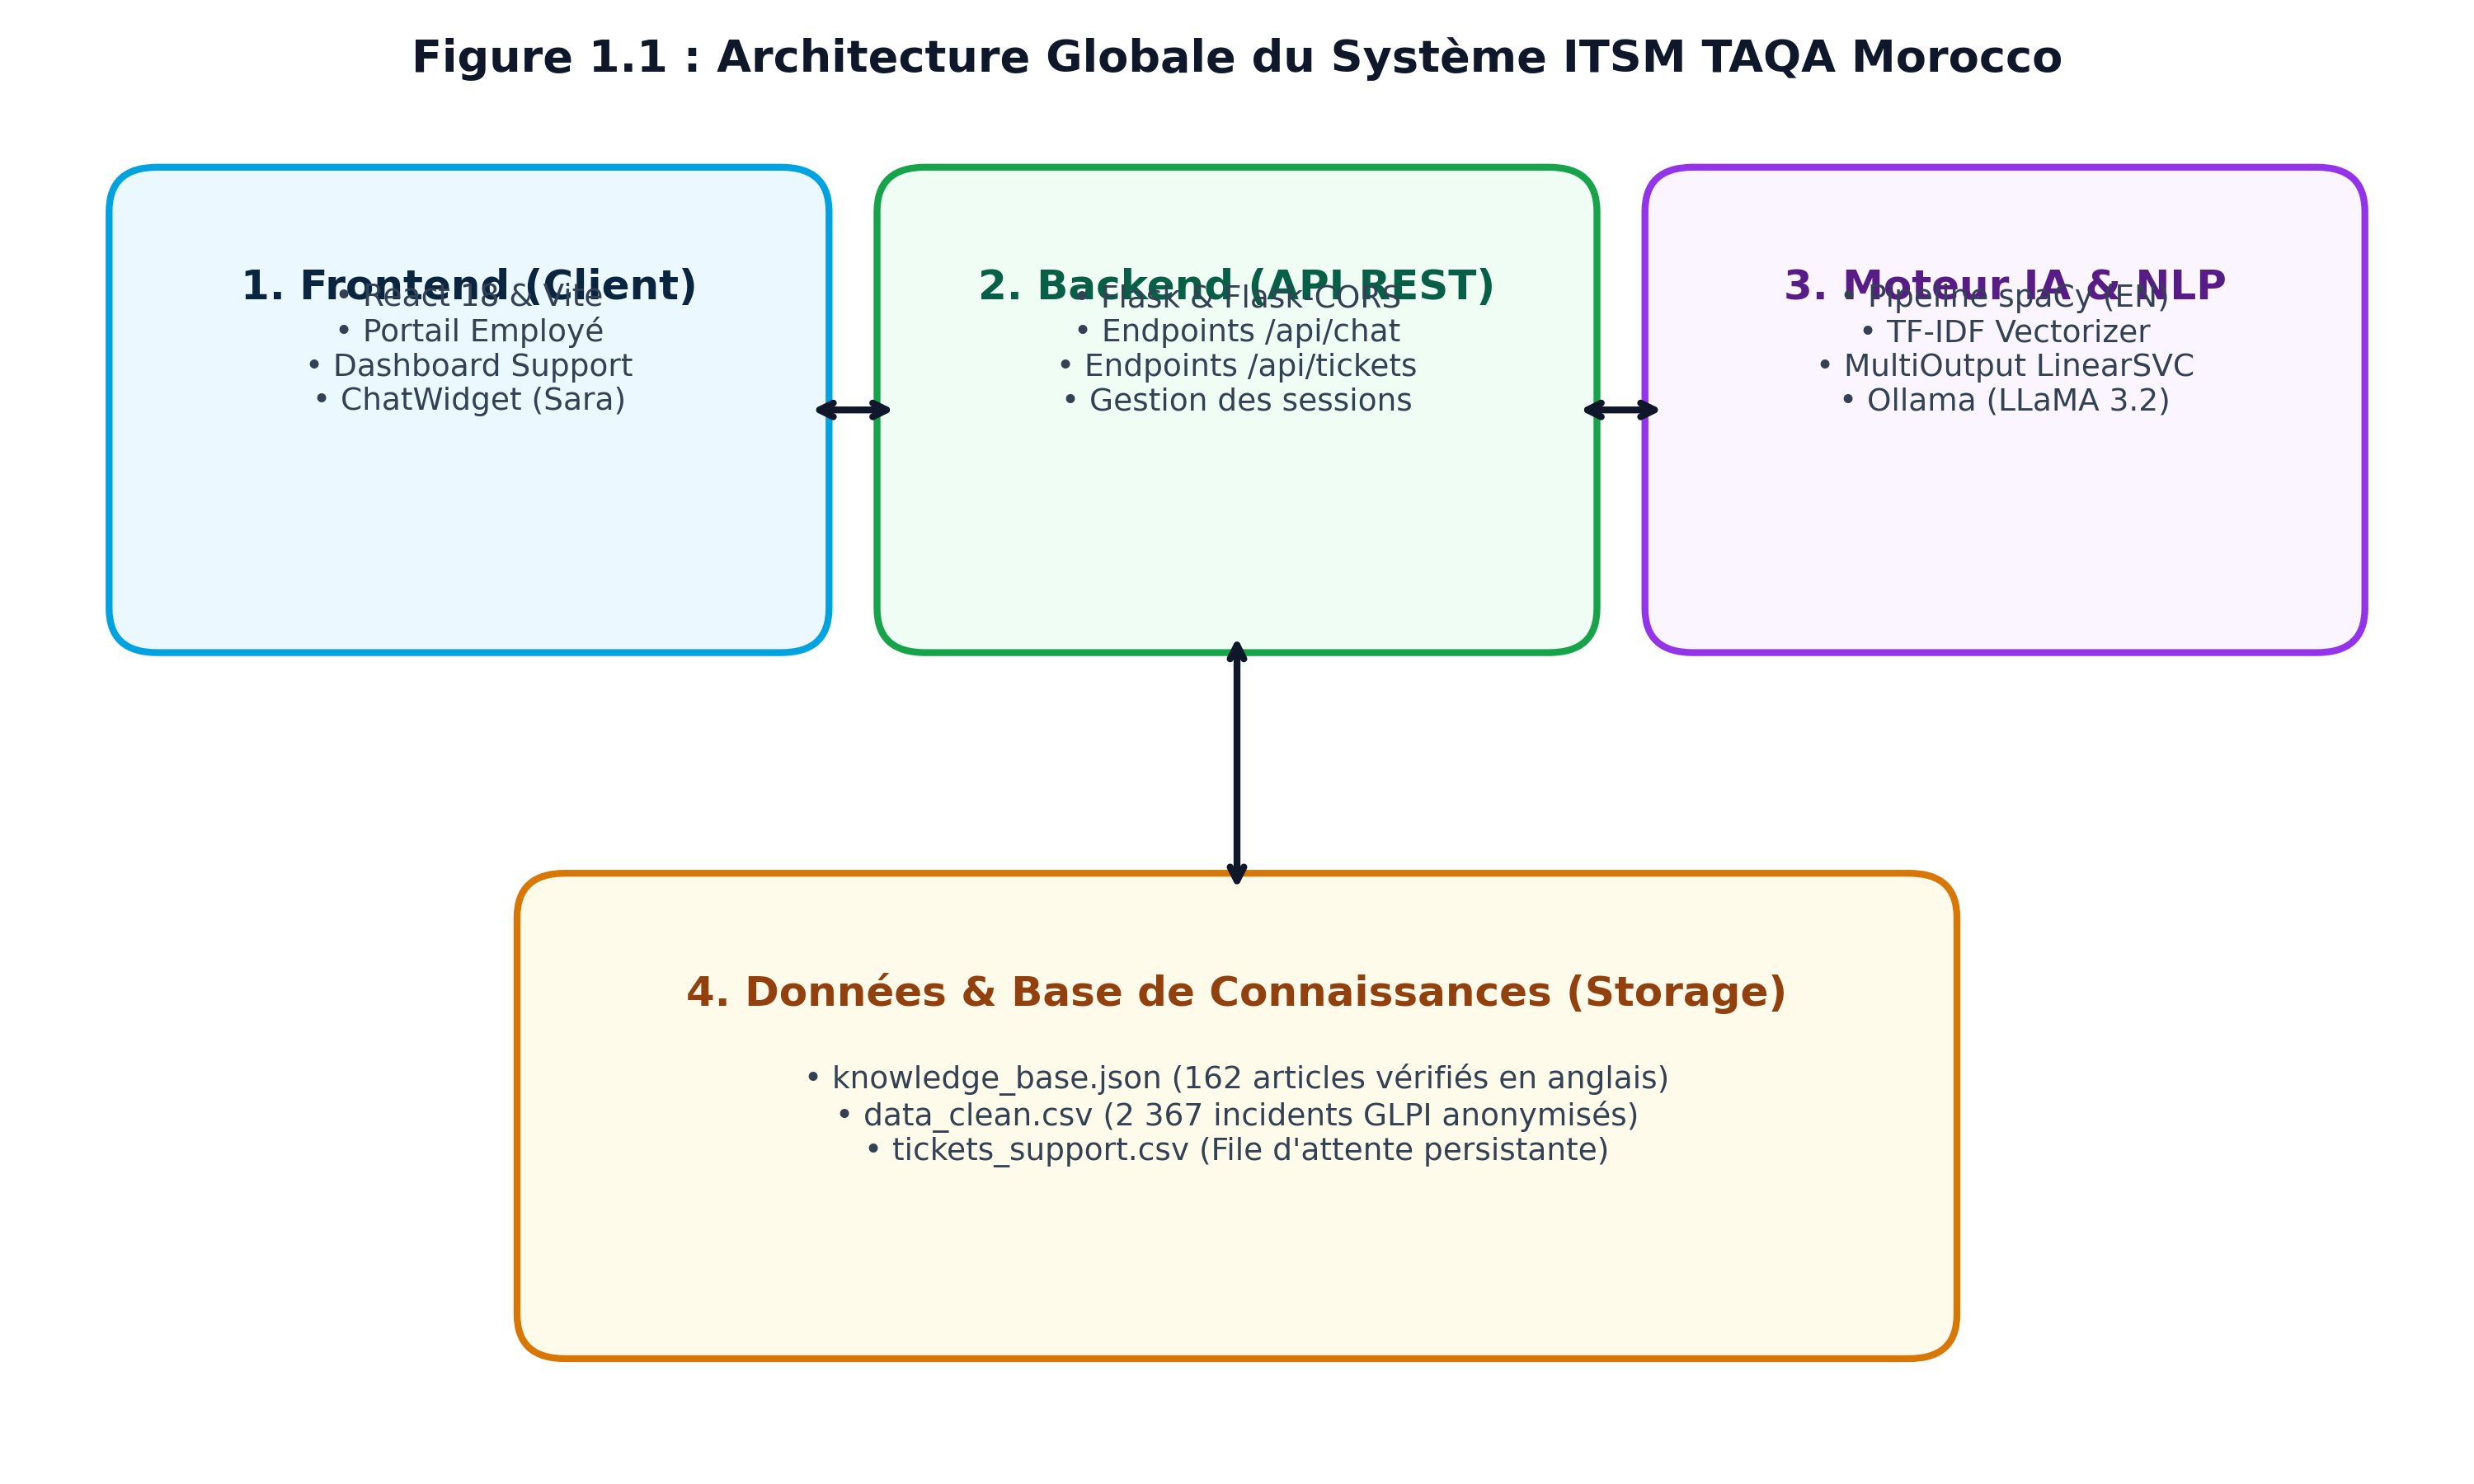
\includegraphics[width=\textwidth,keepaspectratio]{fig_architecture}
  \caption{Architecture globale du systeme ITSM TAQA Morocco}
  \label{fig:architecture}
\end{figure}

\section{Etat de l'art -- ITSM et Intelligence Artificielle}

\begin{table}[H]
\centering
\caption{Comparatif des approches d'assistance ITSM}
\label{tab:etat-art}
\small
\begin{tabularx}{\textwidth}{
  >{\bfseries}p{3.5cm} X X >{\columncolor{taqaNavy!8}}X
}
\toprule
\rowcolor{taqaNavy}
{\color{white}Critere} &
{\color{white}Help Desk Classique} &
{\color{white}Cloud LLM Public} &
{\color{white}TAQA Smart Helpdesk} \\
\midrule
Temps de reponse & Plusieurs heures & $<$ 2\,s & \textbf{$<$ 1,5\,s} \\
\rowcolor{taqaLight}
Precision classification & Aleatoire & Variable & \textbf{98,52\,\%} \\
Aiguillage equipes & Manuel & Non garanti & \textbf{Auto. multi-sorties} \\
\rowcolor{taqaLight}
Confidentialite donnees & Interne mais manuel & Risque exfiltration & \textbf{100\,\% On-Premise} \\
Self-service & FAQ statique & Sans validation & \textbf{162 procedures} \\
\bottomrule
\end{tabularx}
\end{table}

\section{Methodologie adoptee -- Agile Scrum}

Le projet a ete conduit en Sprints de deux semaines (Agile Scrum), favorisant
des cycles iteratifs courts et des demonstrations frequentes aux techniciens.

\section*{Conclusion du chapitre}

Ce chapitre a pose le contexte strategique de TAQA Morocco et justifie
l'architecture hybride retenue. Le chapitre suivant detaille la conception.

%% ═══════════════════════════════════════════════════════════
\chapter{Analyse des Besoins et Conception du Systeme}
%% ═══════════════════════════════════════════════════════════

\section{Introduction}

Ce chapitre formalise les exigences fonctionnelles et non-fonctionnelles avant
d'exposer la conception via les diagrammes UML et l'architecture 3-tiers.

\section{Specification des besoins}

\subsection{Besoins fonctionnels -- Employes}

\begin{itemize}
  \item \textbf{Authentification intuitive} : Acces rapide avec selection de
        profil.
  \item \textbf{Dialogue interactif avec Sara} : Saisie en langage naturel
        et reception immediate des instructions.
  \item \textbf{Formulaire IA en temps reel} : Detection instantanee de la
        categorie et de l'equipe support durant la frappe.
  \item \textbf{Suivi des demandes} : Historique et etat d'avancement des
        tickets personnels.
\end{itemize}

\subsection{Besoins fonctionnels -- Techniciens IT}

\begin{itemize}
  \item \textbf{Tableau de bord de supervision} : Vue centralisee par urgence.
  \item \textbf{Filtrage multicritere} : Tri par equipe (Desktop, Network,
        Security, Application Support).
  \item \textbf{Mise a jour d'etat} : Transition \textit{In Progress}
        $\rightarrow$ \textit{Resolved} en un clic.
\end{itemize}

\subsection{Matrice de tracabilite des exigences}

\begin{table}[H]
\centering
\caption{Matrice de tracabilite des exigences fonctionnelles}
\label{tab:exigences}
\begin{tabularx}{\textwidth}{p{1.6cm} p{5.5cm} p{2cm} X}
\toprule
\rowcolor{taqaNavy}
{\color{white}\bfseries ID} &
{\color{white}\bfseries Designation} &
{\color{white}\bfseries Priorite} &
{\color{white}\bfseries Module} \\
\midrule
EF-01 & Authentification basee sur les roles & Haute & LoginPage / Flask \\
\rowcolor{taqaLight}
EF-02 & Prediction ML en direct (frappe) & Haute & TicketForm / API \\
EF-03 & Recherche deterministe KB (162 articles) & Critique & \texttt{get\_solu()} \\
\rowcolor{taqaLight}
EF-04 & Generation reponses via LLaMA 3.2 & Moyenne & Ollama / LLM \\
EF-05 & Escalade automatique et persistance CSV & Critique & server.py \\
\rowcolor{taqaLight}
EF-06 & Dashboard superviseur filtrable & Haute & SupportDashboard.jsx \\
\bottomrule
\end{tabularx}
\end{table}

\section{Modelisation UML}

\subsection{Diagramme global des cas d'utilisation}

\begin{figure}[H]
  \centering
  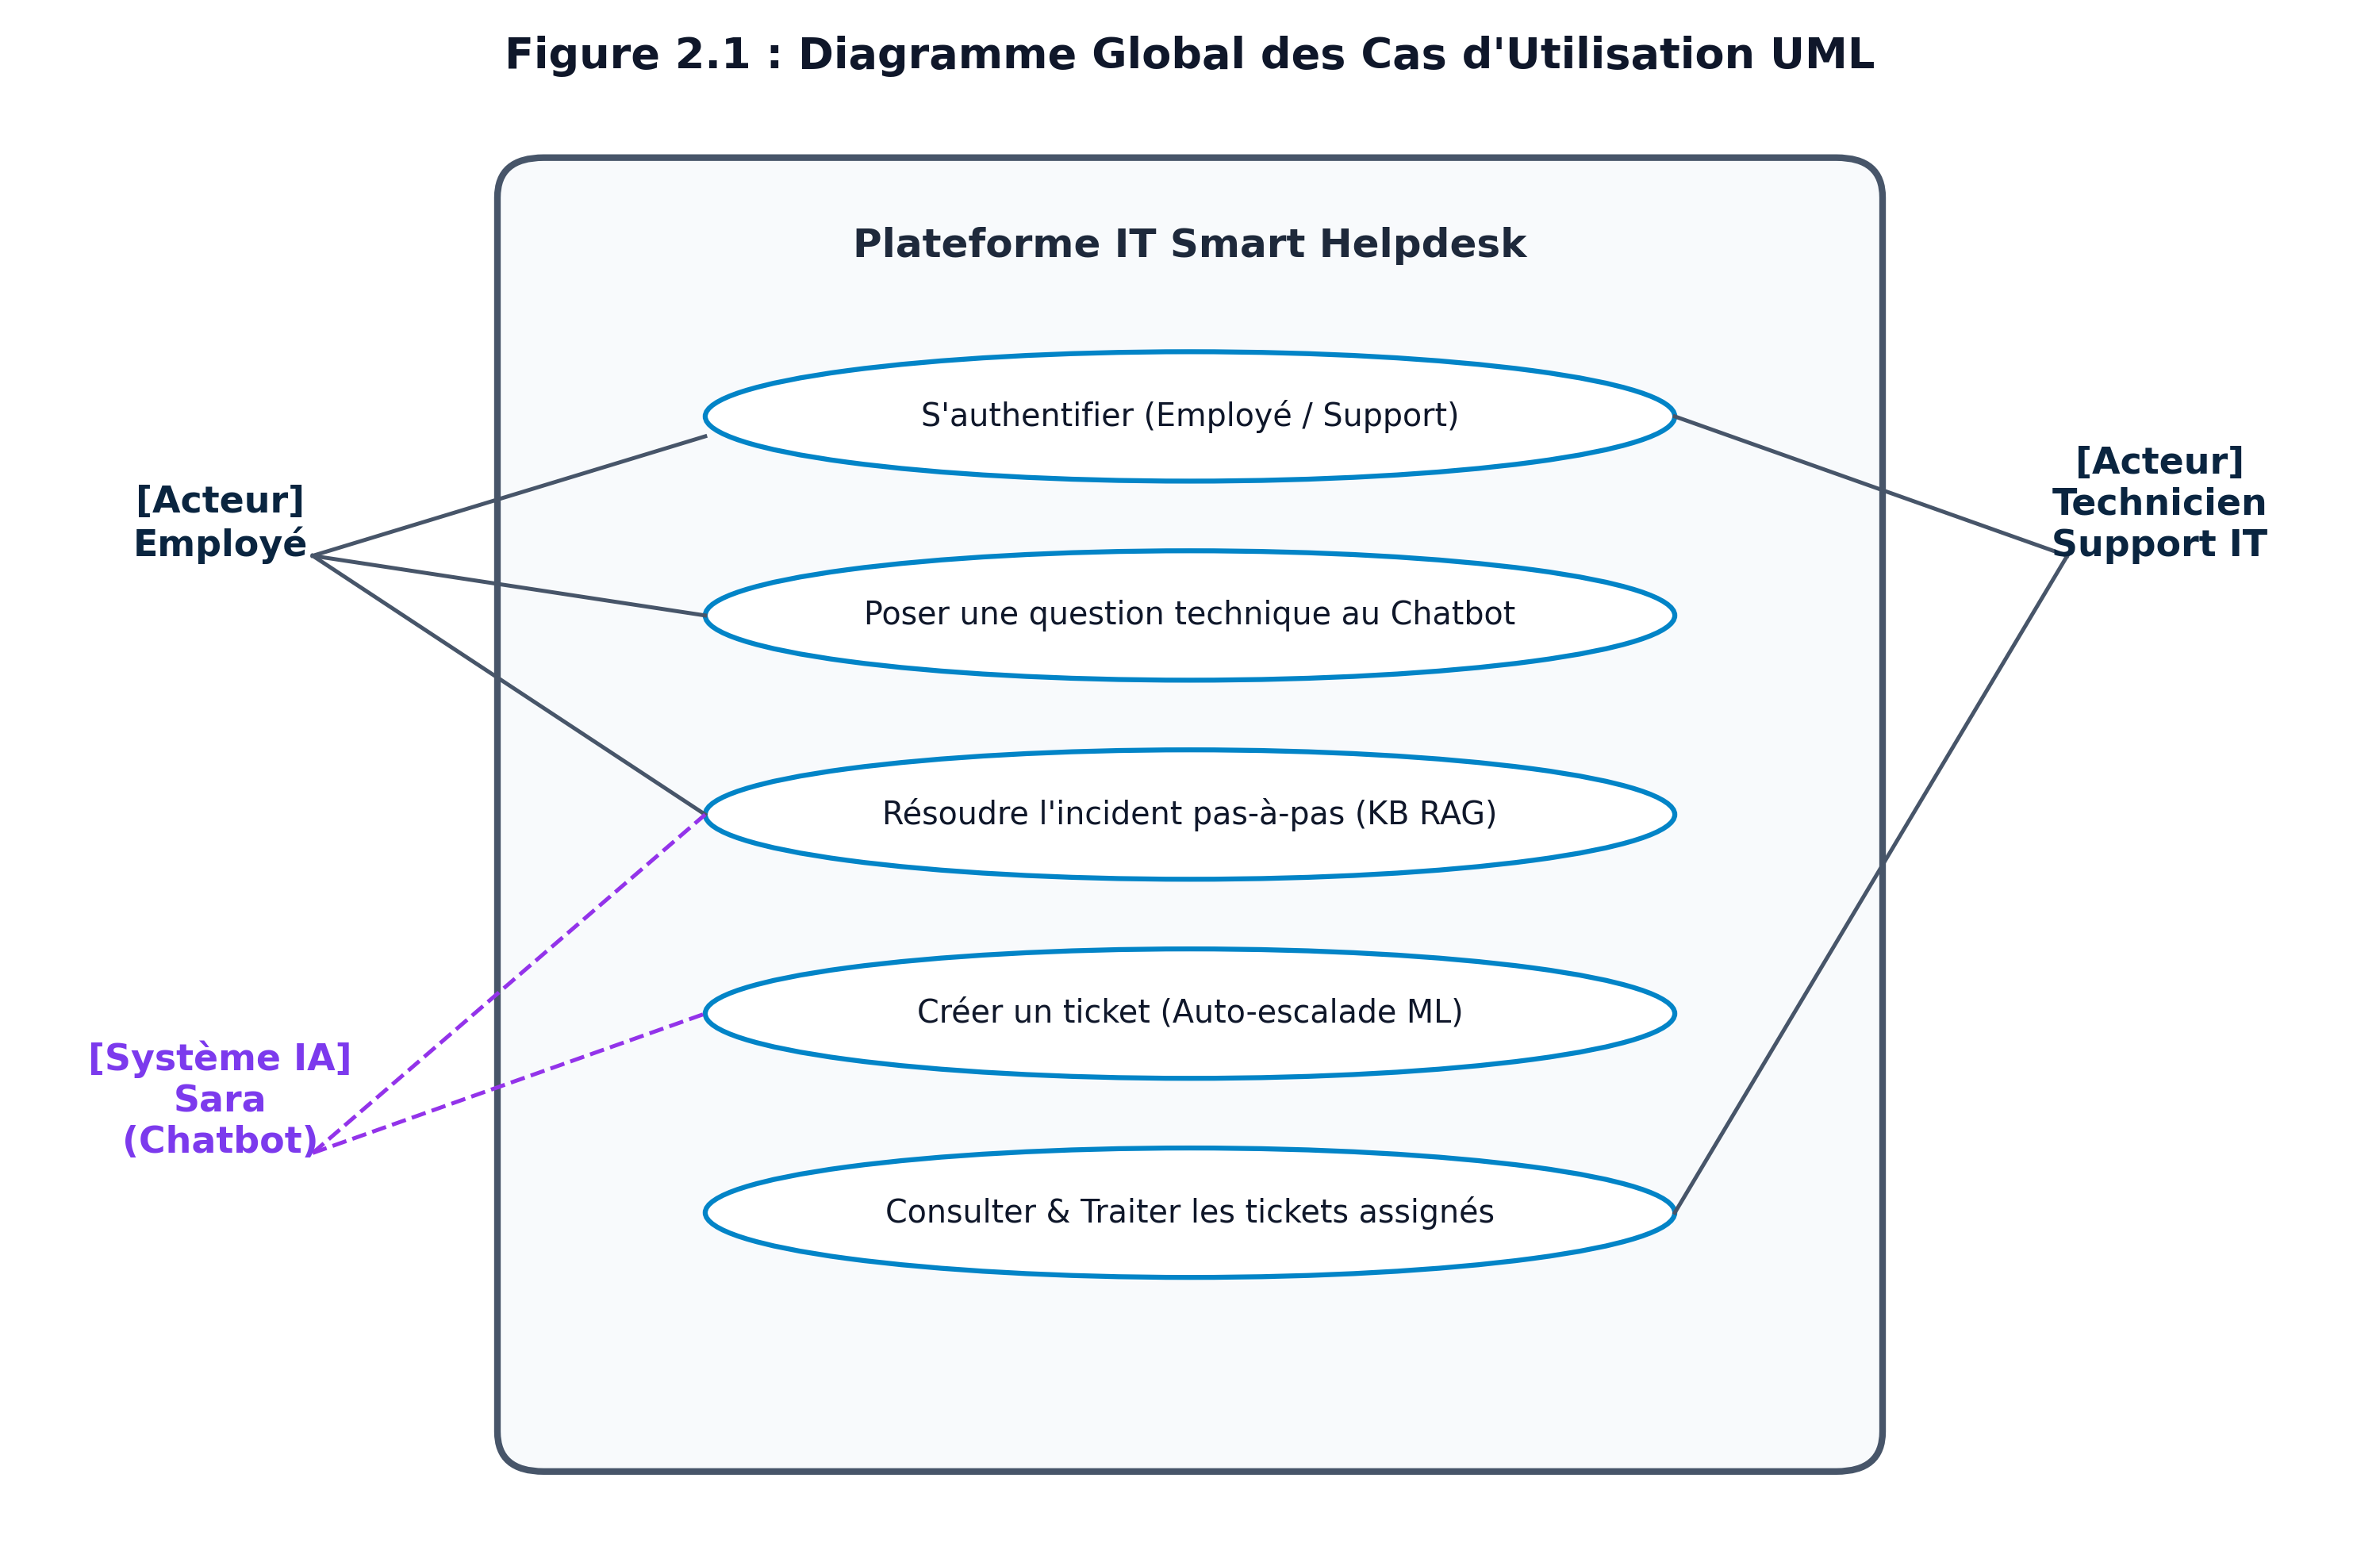
\includegraphics[width=\textwidth,keepaspectratio]{fig_usecase}
  \caption{Diagramme global des cas d'utilisation UML}
  \label{fig:usecase}
\end{figure}

\subsection{Diagramme de sequence -- Resolution par Sara}

\begin{figure}[H]
  \centering
  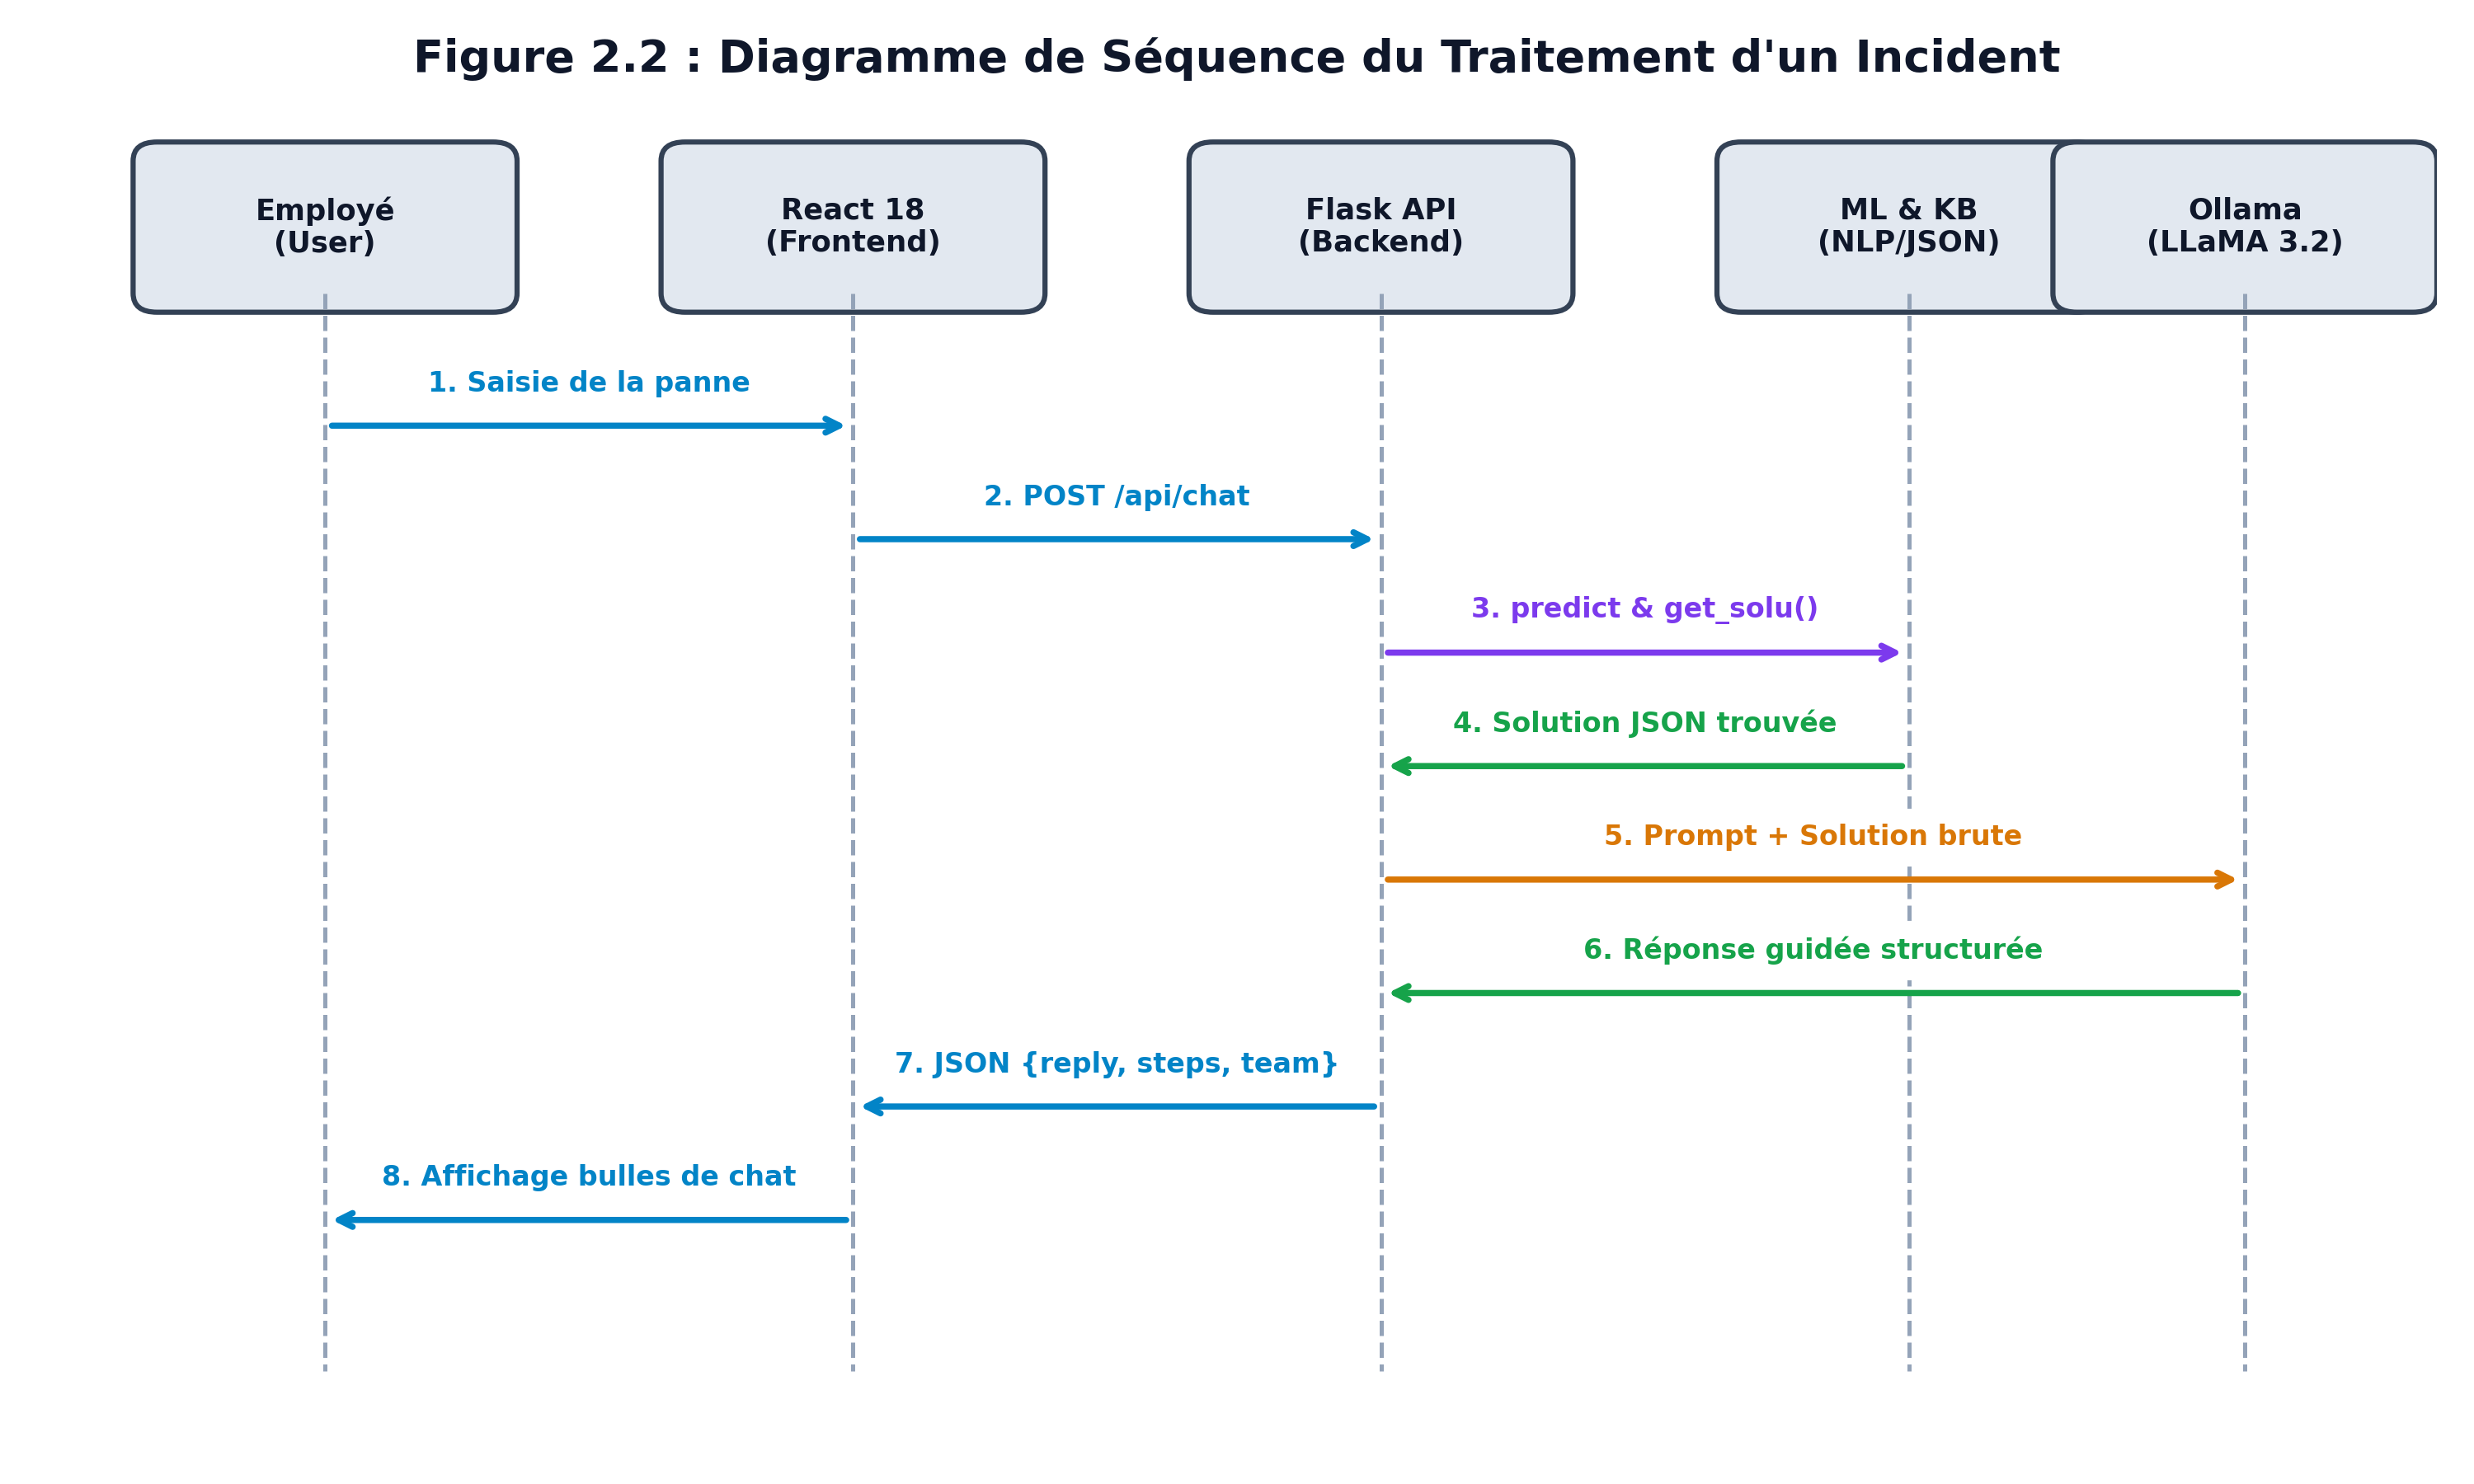
\includegraphics[width=\textwidth,keepaspectratio]{fig_sequence}
  \caption{Diagramme de sequence du traitement d'un incident}
  \label{fig:sequence}
\end{figure}

\subsection{Diagramme d'activite -- Aiguillage intelligent}

\begin{figure}[H]
  \centering
  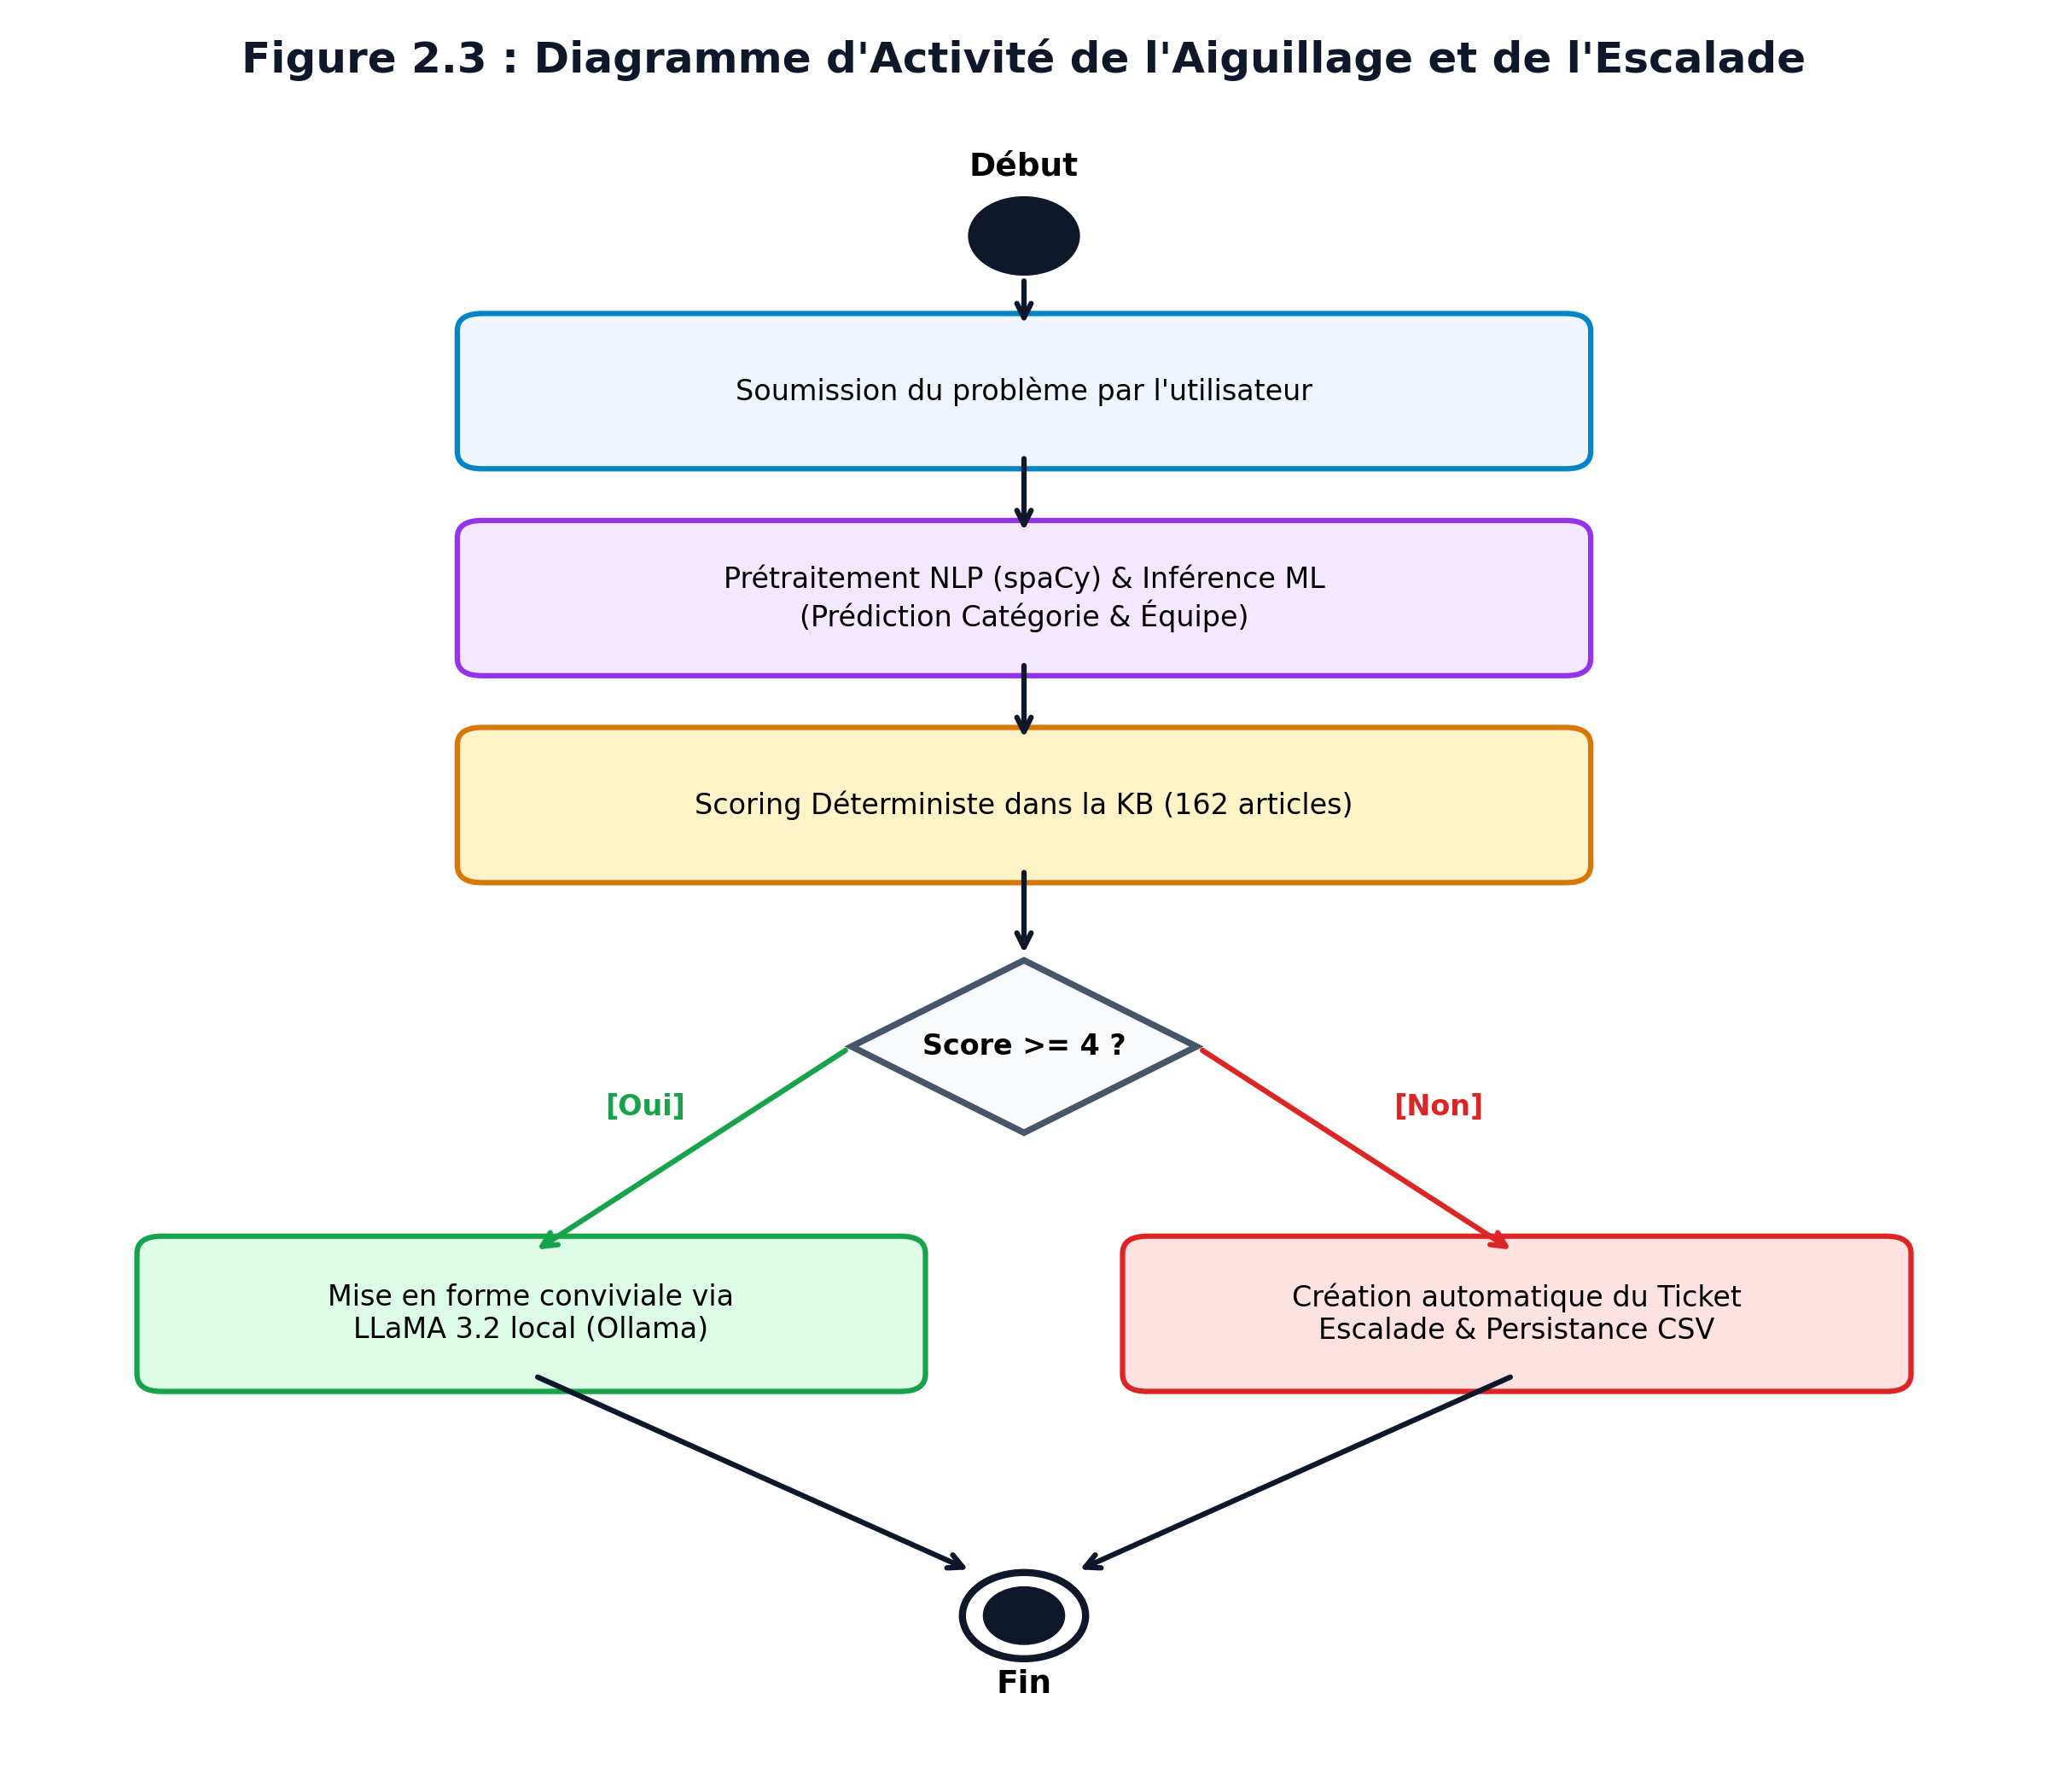
\includegraphics[width=0.88\textwidth,keepaspectratio]{fig_activity}
  \caption{Diagramme d'activite de l'aiguillage et de l'escalade}
  \label{fig:activity}
\end{figure}

\section{Architecture globale 3-tiers}

\begin{tcolorbox}[
  enhanced,
  colback=taqaLight, colframe=taqaNavy,
  title={\textbf{Architecture 3-tiers -- TAQA IT Smart Helpdesk}},
  fonttitle=\bfseries\color{white},
  boxed title style={colback=taqaNavy},
  attach boxed title to top left={yshift=-2mm,xshift=5mm},
]
\begin{description}[leftmargin=2cm]
  \item[\textcolor{taqaCyan}{Couche~1}] \textbf{Presentation (React~18 / Vite)} :
        Interface monopage modulaire avec \texttt{Navbar}, \texttt{TicketForm},
        \texttt{ChatWidget}, \texttt{SupportDashboard}.
  \item[\textcolor{taqaCyan}{Couche~2}] \textbf{Metier \& API (Flask REST)} :
        Controleurs HTTP, orchestration IA, CORS, persistance.
  \item[\textcolor{taqaCyan}{Couche~3}] \textbf{Donnees \& IA} :
        Pipeline spaCy, modeles Scikit-Learn (\texttt{ticket\_pipeline.pkl}),
        JSON (162 solutions), instance Ollama.
\end{description}
\end{tcolorbox}

\section*{Conclusion du chapitre}

Ce chapitre a pose les bases architecturales. Le chapitre suivant aborde le
traitement des donnees GLPI et l'entrainement du modele ML.

%% ═══════════════════════════════════════════════════════════
\chapter{Pretraitement NLP, Pipeline spaCy et Modelisation ML}
%% ═══════════════════════════════════════════════════════════

\section{Introduction}

L'efficacite de l'aiguillage automatique depend de la qualite du pretraitement
linguistique. Ce chapitre expose la preparation du jeu de donnees GLPI (2\,367
incidents), l'anonymisation PII, la vectorisation TF-IDF et l'entrainement du
modele \texttt{MultiOutputClassifier}.

\section{Description du jeu de donnees GLPI (2\,367 tickets)}

\begin{table}[H]
\centering
\caption{Structure et champs du jeu de donnees brut GLPI}
\label{tab:dataset}
\begin{tabularx}{\textwidth}{p{3cm} p{2.8cm} p{4cm} X}
\toprule
\rowcolor{taqaNavy}
{\color{white}\bfseries Champ} &
{\color{white}\bfseries Type} &
{\color{white}\bfseries Description} &
{\color{white}\bfseries Exemple} \\
\midrule
ticket\_id & Entier & Identifiant unique & TCK-1042 \\
\rowcolor{taqaLight}
Description & Texte libre & Incident decrit par l'utilisateur & Cisco AnyConnect error 412 \\
Category & Categorielle (5) & Domaine fonctionnel & Network \\
\rowcolor{taqaLight}
Assigned\_Team & Categorielle (4) & Equipe technique & Network Team \\
Priority & Ordinale (3) & Urgence operationnelle & High \\
\bottomrule
\end{tabularx}
\end{table}

\begin{remarque}
Distribution equilibree : \textit{Network} (510), \textit{Access} (495),
\textit{Hardware} (470), \textit{Security} (452), \textit{Software} (440).
\end{remarque}

\section{Anonymisation PII -- \texttt{cleanup.py}}

\begin{table}[H]
\centering
\caption{Regles de masquage PII appliquees par \texttt{cleanup.py}}
\label{tab:pii}
\begin{tabularx}{\textwidth}{p{3.8cm} p{6cm} X}
\toprule
\rowcolor{taqaNavy}
{\color{white}\bfseries Type de donnee} &
{\color{white}\bfseries Pattern Regex} &
{\color{white}\bfseries Jeton} \\
\midrule
Emails professionnels & \verb|[\w\.-]+@taqa\.ma| & \texttt{[EMAIL]} \\
\rowcolor{taqaLight}
Telephones / Postes & \verb|(\+212|0)[5-7]\d{8}| & \texttt{[PHONE]} \\
Matricules & \verb|(EMP|MAT)[-_]?\d{4,6}| & \texttt{[EMP\_ID]} \\
\rowcolor{taqaLight}
Adresses IP internes & \verb|192\.168\.\d+\.\d+| & \texttt{[IP\_ADDR]} \\
\bottomrule
\end{tabularx}
\end{table}

\section{Traitement linguistique avec spaCy}

Les etapes du pipeline spaCy \texttt{en\_core\_web\_sm} :
\begin{enumerate}
  \item \textbf{Elimination du bruit} : Ponctuation et caracterss speciaux.
  \item \textbf{Filtrage Stopwords} : Pronoms, prepositions, conjonctions.
  \item \textbf{Lemmatisation} : \textit{"connecting"} $\rightarrow$
        \textit{"connect"} ; \textit{"printers"} $\rightarrow$ \textit{"printer"}.
\end{enumerate}

\begin{figure}[H]
  \centering
  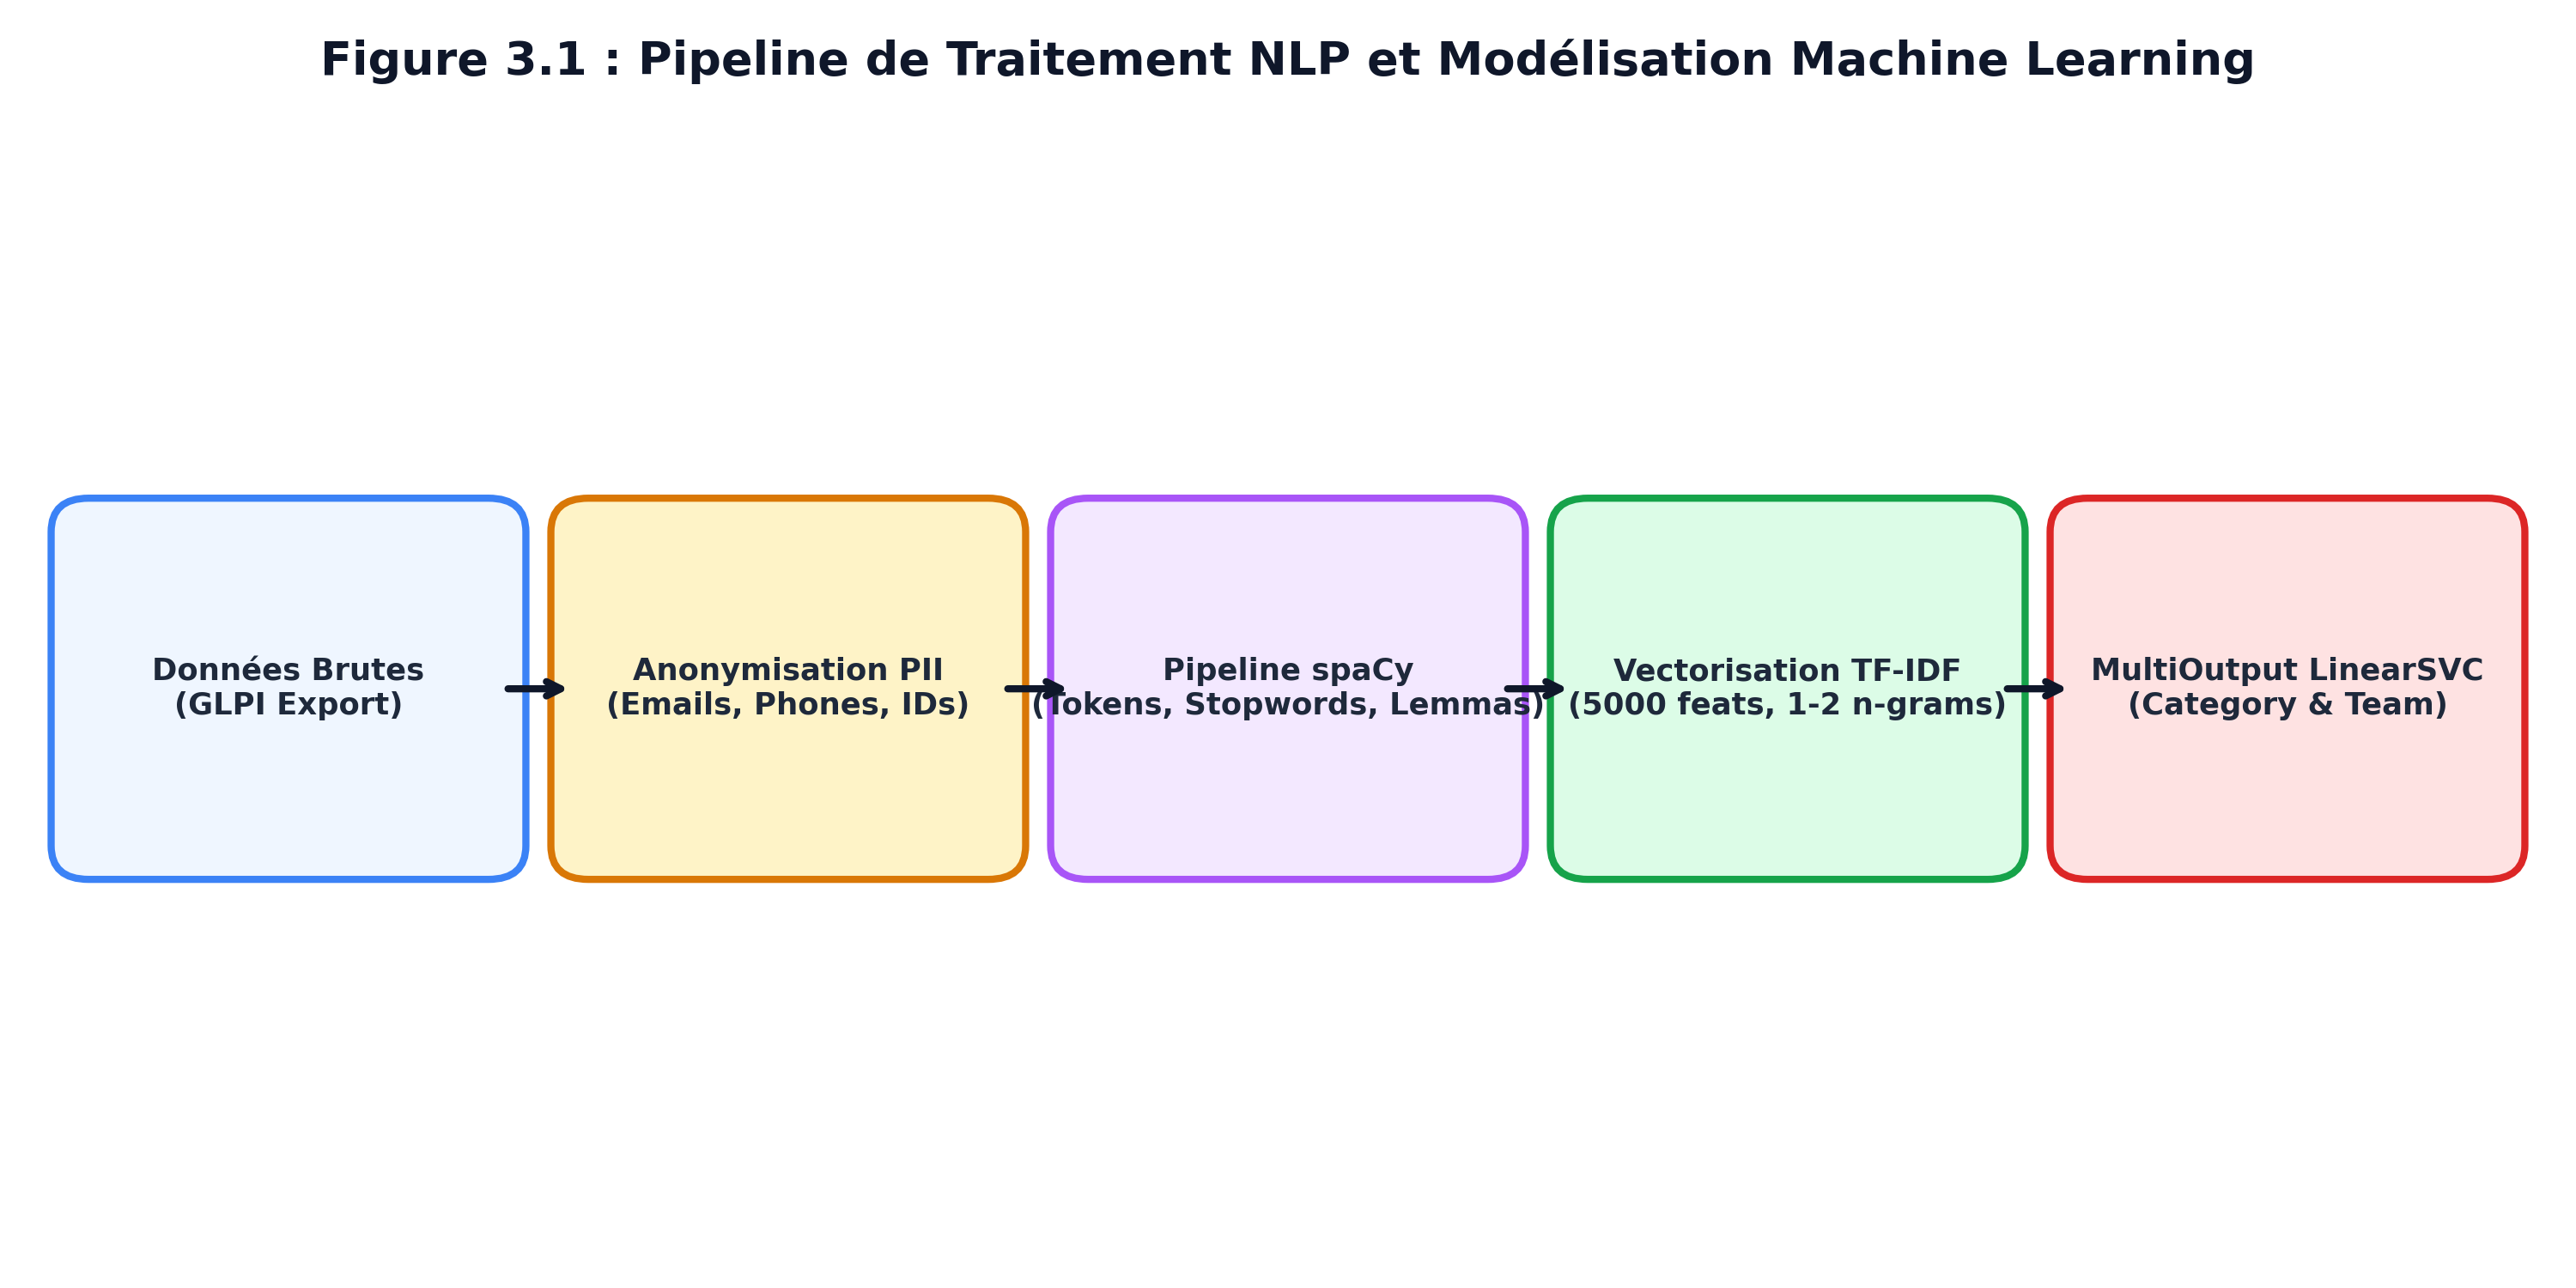
\includegraphics[width=\textwidth,keepaspectratio]{fig_ml_pipeline}
  \caption{Pipeline de traitement NLP et modelisation Machine Learning}
  \label{fig:ml-pipeline}
\end{figure}

\section{Vectorisation TF-IDF}

\begin{equation}
  \text{TF-IDF}(t, d, D) =
  \log(1 + \text{tf}(t,d)) \times
  \log\frac{|D|}{|\{d' \in D : t \in d'\}|}
\end{equation}

\textbf{Parametres optimises :} \texttt{max\_features=5\,000},
\texttt{ngram\_range=(1,2)}, \texttt{sublinear\_tf=True}.

\section{Modelisation predictive multi-sorties}

\subsection{Algorithme LinearSVC et MultiOutputClassifier}

Le classifieur LinearSVC resout le probleme d'optimisation :
\begin{equation}
  \min_{\mathbf{w},b,\xi} \;\frac{1}{2}\|\mathbf{w}\|^2 + C\sum_{i=1}^{n}\xi_i
  \quad \text{s.c.} \quad
  y_i(\mathbf{w}^\top \phi(\mathbf{x}_i) + b) \geq 1 - \xi_i, \;\xi_i \geq 0
\end{equation}

\begin{remarque}
Vitesse d'inference : moins de \textbf{5\,ms} par prediction, permettant la
detection en temps reel durant la frappe dans le formulaire React.
\end{remarque}

\subsection{Entrainement et hyperparametres}

\begin{lstlisting}[style=python,
  caption=Entrainement du modele multi-sorties -- \texttt{src/model.py}]
from sklearn.pipeline import Pipeline
from sklearn.feature_extraction.text import TfidfVectorizer
from sklearn.svm import LinearSVC
from sklearn.multioutput import MultiOutputClassifier
from sklearn.model_selection import GridSearchCV
import joblib

# Construction du pipeline TF-IDF + MultiOutput SVC
pipeline = Pipeline([
    ('tfidf', TfidfVectorizer(
        max_features=5000,
        ngram_range=(1, 2),
        sublinear_tf=True
    )),
    ('clf', MultiOutputClassifier(
        LinearSVC(max_iter=2000)
    ))
])

# Optimisation des hyperparametres par GridSearchCV (3 plis)
param_grid = {
    'clf__estimator__C': [0.1, 1.0, 5.0, 10.0],
    'clf__estimator__class_weight': [None, 'balanced']
}
grid = GridSearchCV(pipeline, param_grid,
                    cv=3, scoring='f1_weighted', n_jobs=-1)
grid.fit(X_train, Y_train)  # Y_train : [Category, Assigned_Team]

# Serialisation du meilleur modele
joblib.dump(grid.best_estimator_, 'models/ticket_pipeline.pkl')
print(f"Best params: {grid.best_params_}")
print(f"Best F1: {grid.best_score_:.4f}")
\end{lstlisting}

\section{Resultats experimentaux}

\begin{resultat}
\begin{center}
  \begin{tabular}{lc}
    \toprule
    \textbf{Metrique} & \textbf{Score} \\
    \midrule
    Exactitude Categorie & \textbf{98,52\,\%} \\
    Exactitude Equipe Assignee & \textbf{98,52\,\%} \\
    Exact Match Ratio (conjointe) & \textbf{98,52\,\%} \\
    F1-Score moyen pondere & \textbf{0,99} \\
    Taille jeu de test & 474 tickets (20\,\%) \\
    \bottomrule
  \end{tabular}
\end{center}
\end{resultat}

\begin{table}[H]
\centering
\caption{Rapport de classification par Categorie (Test Set -- 474 tickets)}
\label{tab:classif-cat}
\begin{tabular}{lcccr}
\toprule
\rowcolor{taqaNavy}
{\color{white}\bfseries Categorie} &
{\color{white}\bfseries Precision} &
{\color{white}\bfseries Rappel} &
{\color{white}\bfseries F1-Score} &
{\color{white}\bfseries Support} \\
\midrule
Access   & 0,99 & 0,97 & 0,98 & 101 \\
\rowcolor{taqaLight}
Hardware & 1,00 & 1,00 & \textbf{1,00} & 92 \\
Network  & 0,97 & 1,00 & 0,99 & 104 \\
\rowcolor{taqaLight}
Security & 0,97 & 1,00 & 0,98 & 89 \\
Software & 1,00 & 0,95 & 0,98 & 88 \\
\midrule
\textbf{Moy. ponderee} & \textbf{0,99} & \textbf{0,99} &
\textbf{0,99} & \textbf{474} \\
\bottomrule
\end{tabular}
\end{table}

\begin{table}[H]
\centering
\caption{Rapport de classification par Equipe Support (Test Set -- 474 tickets)}
\label{tab:classif-team}
\begin{tabular}{lcccr}
\toprule
\rowcolor{taqaNavy}
{\color{white}\bfseries Equipe Support} &
{\color{white}\bfseries Precision} &
{\color{white}\bfseries Rappel} &
{\color{white}\bfseries F1-Score} &
{\color{white}\bfseries Support} \\
\midrule
Application Support & 1,00 & 0,97 & 0,98 & 125 \\
\rowcolor{taqaLight}
Desktop Support     & 0,99 & 0,99 & 0,99 & 156 \\
Network Team        & 0,97 & 1,00 & 0,99 & 104 \\
\rowcolor{taqaLight}
Security Team       & 0,97 & 1,00 & 0,98 & 89 \\
\midrule
\textbf{Moy. ponderee} & \textbf{0,98} & \textbf{0,99} &
\textbf{0,99} & \textbf{474} \\
\bottomrule
\end{tabular}
\end{table}

\begin{figure}[H]
  \centering
  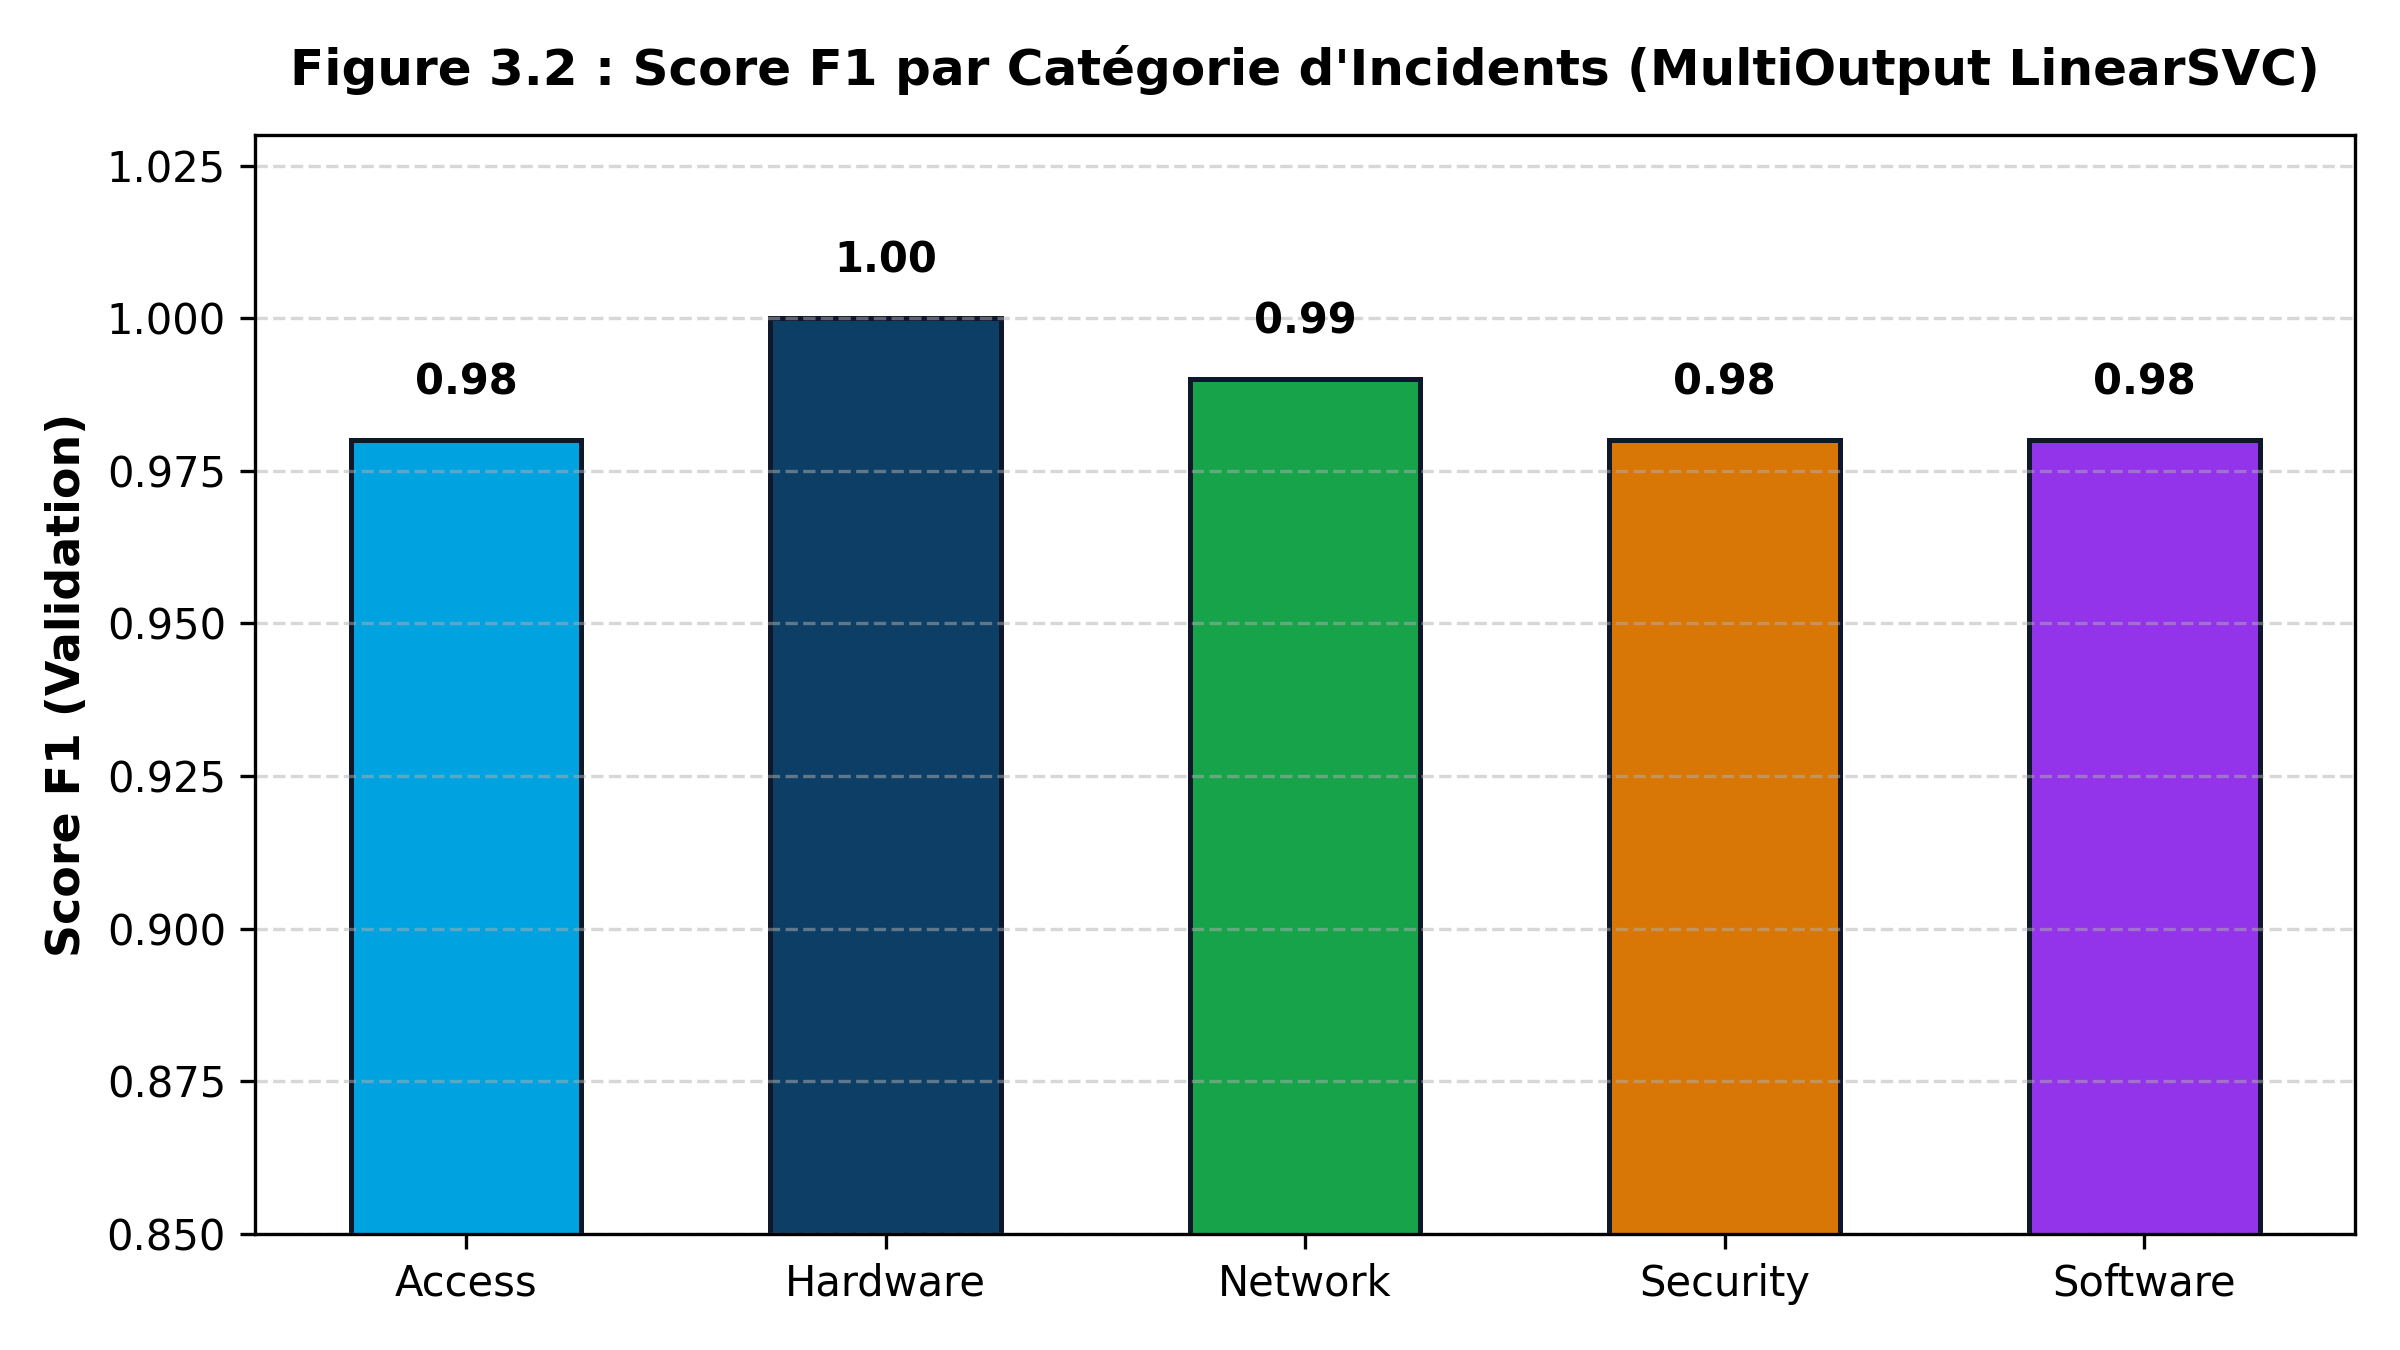
\includegraphics[width=0.85\textwidth,keepaspectratio]{fig_ml_performance}
  \caption{Score F1 par categorie d'incidents -- MultiOutput LinearSVC}
  \label{fig:ml-performance}
\end{figure}

\section*{Conclusion du chapitre}

Le pipeline NLP spaCy + LinearSVC multi-sorties atteint \textbf{98,52\,\%}
de precision. Le chapitre suivant traite le moteur RAG et LLaMA 3.2.

%% ═══════════════════════════════════════════════════════════
\chapter{Moteur RAG Deterministe, Agent LLM et Base de Connaissances}
%% ═══════════════════════════════════════════════════════════

\section{Introduction}

Ce chapitre presente la base de connaissances de 162 articles, l'algorithme
de recherche deterministe, l'integration locale de LLaMA 3.2 via Ollama et
le mecanisme d'escalade automatique des tickets.

\section{Base de connaissances IT -- 162 solutions}

\subsection{Taxonomie et repartition}

\begin{table}[H]
\centering
\caption{Repartition des 162 procedures par equipe technique}
\label{tab:kb-repartition}
\begin{tabularx}{\textwidth}{p{4.5cm} c X}
\toprule
\rowcolor{taqaNavy}
{\color{white}\bfseries Equipe} &
{\color{white}\bfseries Fiches} &
{\color{white}\bfseries Thematiques couvertes} \\
\midrule
Desktop Support & 63 & BitLocker, ecrans multiples, docks Dell, imprimantes \\
\rowcolor{taqaLight}
Application Support \& SAP & 53 & Autorisations SU53, SM12, SP01, SAP GUI, Teams \\
Security Team & 25 & Ransomware, EDR Falcon, DLP USB, phishing \\
\rowcolor{taqaLight}
Network Team & 21 & VPN AnyConnect, Wi-Fi 802.1X, conflits IP, OT \\
\midrule
\textbf{Total} & \textbf{162} & \\
\bottomrule
\end{tabularx}
\end{table}

\subsection{Structure normalisee des fiches JSON}

\begin{lstlisting}[style=python,
  caption=Exemple de fiche technique JSON -- \texttt{knowledge\_base.json}]
{
  "Category": "Access",
  "Assigned_Team": "Desktop Support",
  "Problem_Title": "Corporate Password Reset Procedure",
  "Keywords": [
    "password", "mot de passe", "reset", "forgotten",
    "locked", "bloque", "password expired", "kbir"
  ],
  "Requires_Escalation": false,
  "Chatbot_Response": "## Password Reset Procedure\n\n
    1. Open your browser: https://portal.taqa.ma/reset\n
    2. Enter your professional email (nom.prenom@taqa.ma)\n
    3. Check inbox for secure link from noreply@taqa.ma\n
    4. Choose a strong password:\n
       - Minimum 12 characters\n
       - 1 uppercase, 1 lowercase, 1 digit, 1 special char\n
    5. Lock session (Ctrl+Alt+Del) and unlock with new password."
}
\end{lstlisting}

\section{Moteur de recherche deterministe -- \texttt{get\_solu()}}

\begin{table}[H]
\centering
\caption{Bareme de scoring du moteur de recherche deterministe}
\label{tab:scoring}
\begin{tabularx}{\textwidth}{p{5cm} X p{2.5cm}}
\toprule
\rowcolor{taqaNavy}
{\color{white}\bfseries Type de correspondance} &
{\color{white}\bfseries Regle} &
{\color{white}\bfseries Poids} \\
\midrule
Mot-cle long ($>$ 6 chars) & Correspondance exacte avec \verb|\b| & $+4$ pts \\
\rowcolor{taqaLight}
Mot-cle court ($\leq$ 6 chars) & Correspondance exacte & $+2$ pts \\
Terme commun dans le titre & Mot pertinent partage (hors stopwords) & $+5$ pts \\
\rowcolor{taqaLight}
Bonus Categorie ML & Concordance avec prediction LinearSVC & $+3$ pts \\
Seuil minimal & Score cumulé minimal d'acceptation & $\geq 4$ pts \\
\bottomrule
\end{tabularx}
\end{table}

\begin{lstlisting}[style=python,
  caption=Algorithme de recherche deterministe -- \texttt{src/utils.py}]
def get_solu(user_msg: str, category: str = None,
             json_path: str = None) -> dict:
    kb   = load_knowledge_base(json_path)
    user_norm = _normalize(user_msg)
    cat_clean = category.strip().lower() if category else ""
    scored = []

    for sol in kb:
        kw_score = 0
        for key in sol.get("Keywords", []):
            k = _normalize(str(key))
            if re.search(r'\b' + re.escape(k) + r'\b', user_norm):
                kw_score += 4 if len(k) > 6 else 2

        # Matching sur les termes du titre (>=4 chars, hors stopwords)
        common = (
            set(re.findall(r'\b\w{4,}\b', user_norm)) &
            set(re.findall(r'\b\w{4,}\b',
                _normalize(sol.get("Problem_Title", ""))))
        )
        title_score = len(common) * 5
        cat_bonus   = 3 if (cat_clean and
                            sol.get("Category","").lower() == cat_clean) else 0
        total = kw_score + title_score + cat_bonus

        if total >= 4:
            scored.append((total, sol))

    if not scored:
        return {"status": "not_found", "needs_escalation": True}

    scored.sort(key=lambda x: x[0], reverse=True)
    best = scored[0][1]
    return {
        "status":        "success",
        "chatbot_reply": best.get("Chatbot_Response"),
        "category":      best.get("Category"),
        "assigned_team": best.get("Assigned_Team"),
        "problem_title": best.get("Problem_Title"),
    }
\end{lstlisting}

\section{Agent conversationnel LLaMA 3.2 via Ollama}

\begin{figure}[H]
  \centering
  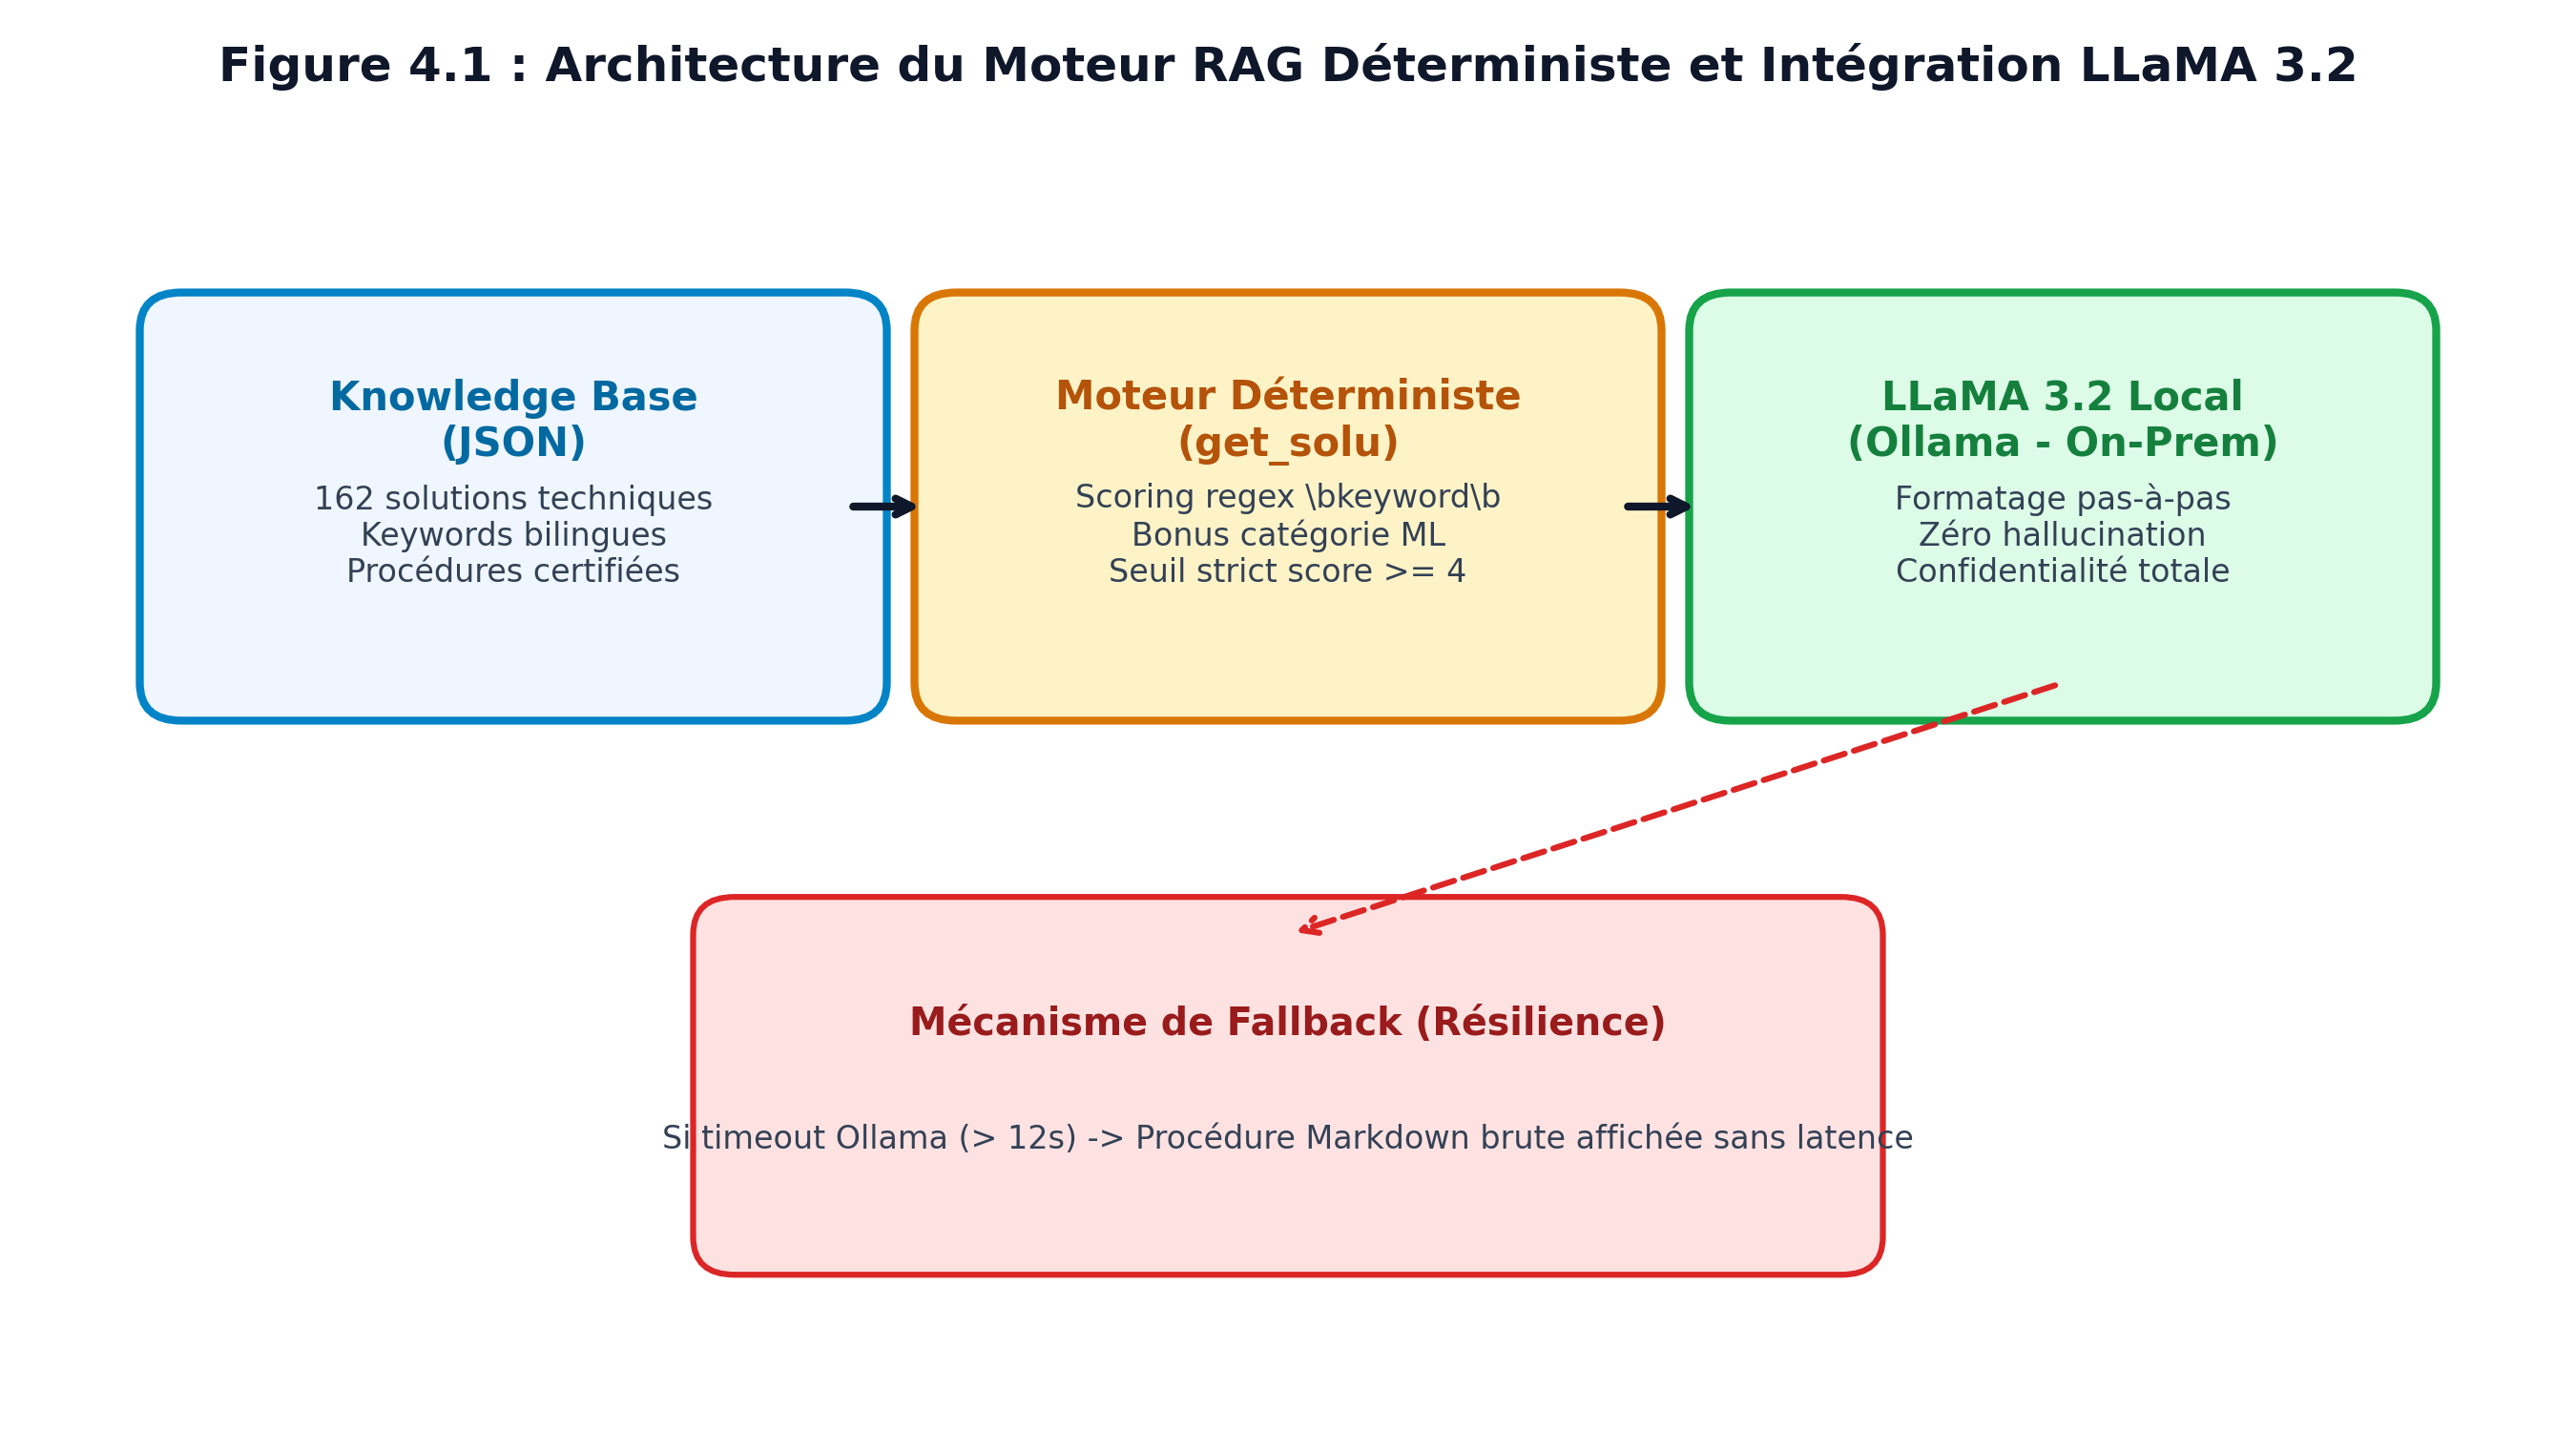
\includegraphics[width=\textwidth,keepaspectratio]{fig_rag_ollama}
  \caption{Architecture du moteur RAG deterministe et integration LLaMA 3.2}
  \label{fig:rag-ollama}
\end{figure}

\subsection{Integration souveraine On-Premise}

Aucun texte d'incident n'est envoye vers des services cloud externes. Nous
exploitons \textbf{LLaMA 3.2 (3 milliards de parametres)} heberge localement
via \textbf{Ollama} (port 11434). La confidentialite est garantie
conformement aux exigences CNDP et DGSSI.

\subsection{Role et Prompt Engineering de l'agente Sara}

Le LLM agit comme un \textbf{transformateur d'experience utilisateur} :
\begin{itemize}
  \item Reformule la procedure brute JSON avec bienveillance et clarte.
  \item Decoupe les actions en etapes sequentielles numerotees.
  \item Preserve les commandes, adresses IP et URLs corporatives.
  \item Conclut en demandant si le probleme est resolu.
\end{itemize}

\subsection{Resilience -- Mecanisme de fallback (timeout 12 s)}

Un thread asynchrone surveille l'appel Ollama. En cas de depassement du
timeout de \textbf{12 secondes}, la fonction \texttt{\_simplified\_response()}
affiche directement la procedure Markdown sans interruption.

\section{Mecanisme d'escalade automatique}

Lorsqu'un probleme inedite est soumis (score $< 4$) ou qu'une assistance
humaine est demandee, la plateforme :
\begin{enumerate}
  \item Cree automatiquement un ticket numerote (ex: \texttt{TCK-1008}).
  \item Assigne a l'equipe predite par \texttt{predict\_category\_and\_team()}.
  \item Estime la priorite (\textit{Critical} si urgence, \textit{High} pour
        Reseau / Securite, \textit{Normal} par defaut).
  \item Persiste dans \texttt{tickets\_support.csv} et alerte le technicien.
\end{enumerate}

\section*{Conclusion du chapitre}

La synergie entre 162 solutions certifiees, le moteur deterministe sans
hallucination et la fluidite de LLaMA 3.2 forme un systeme fiable et souverain.

%% ═══════════════════════════════════════════════════════════
\chapter{Realisation, Interfaces et Deploiement}
%% ═══════════════════════════════════════════════════════════

\section{Introduction}

Ce chapitre illustre les interfaces React~18, la charte visuelle TAQA, les
tests d'integration et les scripts de deploiement.

\section{Environnement technique}

\begin{table}[H]
\centering
\caption{Pile logicielle et versions des technologies deployees}
\label{tab:stack}
\begin{tabularx}{\textwidth}{p{3.5cm} p{3.5cm} p{2.5cm} X}
\toprule
\rowcolor{taqaNavy}
{\color{white}\bfseries Composant} &
{\color{white}\bfseries Technologie} &
{\color{white}\bfseries Version} &
{\color{white}\bfseries Role} \\
\midrule
Frontend SPA & React \& Vite & 18.3 / 6.0 & Interface monopage reactive \\
\rowcolor{taqaLight}
Styles CSS & Vanilla CSS3 / Tokens & CSS Custom Props & Glassmorphism TAQA \\
Backend API & Python Flask & 3.1 / Python 3.13 & REST, orchestration IA \\
\rowcolor{taqaLight}
Pipeline NLP & spaCy & 3.8.4 & Tokenisation, lemmatisation \\
ML & Scikit-Learn \& Joblib & 1.6 & TF-IDF, MultiOutput SVC \\
\rowcolor{taqaLight}
Agent LLM & Ollama / LLaMA 3.2 & 0.6 / 3B params & Dialogue On-Premise \\
Base conn. & JSON structure & UTF-8 & 162 fiches d'assistance \\
\bottomrule
\end{tabularx}
\end{table}

\section{Interfaces utilisateurs}

\subsection{Authentification -- \texttt{LoginPage.jsx}}

Design epure avec logo officiel TAQA sur fond degrade bleu nuit. L'utilisateur
choisit son profil (\textit{Employe} ou \textit{Technicien Support}) avec
selection optionnelle de l'equipe d'affectation.

\subsection{Portail Employe -- \texttt{TicketForm.jsx}}

\begin{itemize}
  \item Cartes de statistiques personnelles (Tickets declares, En cours, Resolus).
  \item \textbf{Formulaire IA en temps reel} : prediction de categorie et equipe
        affichees durant la frappe (appel API \texttt{/api/predict} a chaque
        keystroke avec debounce 500\,ms).
  \item Tableau recapitulatif des incidents mis a jour en direct.
\end{itemize}

\subsection{Widget conversationnel Sara -- \texttt{ChatWidget.jsx}}

\begin{itemize}
  \item Bouton flottant accessible depuis toutes les pages.
  \item Puces de suggestions rapides : \textit{Password Reset}, \textit{VPN},
        \textit{HELP / Technicien}.
  \item Fil de discussion avec affichage Markdown des etapes de resolution.
  \item Cartes visuelles de confirmation de ticket en cas d'escalade.
\end{itemize}

\subsection{Tableau de bord Superviseur -- \texttt{SupportDashboard.jsx}}

\begin{itemize}
  \item Vue filtrable par equipe (4 equipes distinctes).
  \item Badges de statut interactifs (\textit{In Progress}
        $\rightarrow$ \textit{Resolved}) en un clic.
  \item Indicateurs de priorite visuels (Critical, High, Normal).
\end{itemize}

\section{Tests d'integration et validation}

\begin{table}[H]
\centering
\caption{Synthese des scenarios de validation fonctionnelle}
\label{tab:tests}
\begin{tabularx}{\textwidth}{p{0.8cm} p{3.8cm} p{4cm} X}
\toprule
\rowcolor{taqaNavy}
{\color{white}\bfseries N} &
{\color{white}\bfseries Requete testee} &
{\color{white}\bfseries Comportement attendu} &
{\color{white}\bfseries Resultat} \\
\midrule
1 & VPN split tunneling & Solution N121 -- etapes Cisco & \textcolor{taqaCyan}{\bfseries OK} (1,4\,s) \\
\rowcolor{taqaLight}
2 & SAP SU53 authorization & Procedure log SU53 guidee & \textcolor{taqaCyan}{\bfseries OK} \\
3 & Erreur ecran vert 0x883719 & Ticket auto. cree & \textcolor{taqaCyan}{\bfseries OK} (TCK-1009) \\
\rowcolor{taqaLight}
4 & Fichiers chiffres ransomware & Ticket Security Critical & \textcolor{taqaCyan}{\bfseries OK} (escalade) \\
\bottomrule
\end{tabularx}
\end{table}

\section{Deploiement -- \texttt{run\_project.bat}}

\begin{lstlisting}[style=bash,
  caption=Script de demarrage automatise pour Windows -- \texttt{run\_project.bat}]
@echo off
title TAQA IT Smart Helpdesk -- Launcher
color 1F
echo =========================================
echo  TAQA IT Smart Helpdesk -- All Services
echo =========================================

:: Serveur Flask REST API (port 5000)
start "Flask API Backend" cmd /k "py server.py"
timeout /t 3 /nobreak > nul

:: Serveur React Vite (port 5173)
cd frontend
start "React Vite Frontend" cmd /k "npm run dev"

:: Ouverture navigateur automatique
timeout /t 5 /nobreak > nul
start http://localhost:5173

echo.
echo  Backend  : http://localhost:5000
echo  Frontend : http://localhost:5173
echo  Pret !
\end{lstlisting}

\section*{Conclusion du chapitre}

L'application web rapide, intuitive et securisee repond parfaitement aux
exigences operationnelles de TAQA Morocco.

%% ═══════════════════════════════════════════════════════════
%%  CONCLUSION GENERALE
%% ═══════════════════════════════════════════════════════════
\chapter*{Conclusion Generale et Perspectives}
\addcontentsline{toc}{chapter}{Conclusion Generale et Perspectives}
\markboth{Conclusion Generale}{Conclusion Generale}

Ce Projet de Fin d'Annee s'inscrit au coeur de la modernisation des services
informatiques de \textbf{TAQA Morocco}. Nous avons concu, implemente et valide
une solution ITSM complete alliant intelligence predictive, NLP et dialogue
guide autonome.

\begin{tcolorbox}[
  enhanced, breakable,
  colback=taqaNavy!5, colframe=taqaNavy,
  title={\textbf{Bilan des realisations techniques}},
  fonttitle=\bfseries\color{white},
  boxed title style={colback=taqaNavy},
  attach boxed title to top left={yshift=-2mm,xshift=5mm},
]
\begin{itemize}
  \item \textbf{Modele ML haute precision} : MultiOutputClassifier (LinearSVC)
        + TF-IDF bigrammes $\rightarrow$ \textbf{98,52\,\%} de precision conjointe
        sur 2\,367 tickets, eliminant les reassignations manuelles.
  \item \textbf{Moteur RAG deterministe} : 162 procedures certifiees + LLaMA 3.2
        On-Premise $\rightarrow$ resolution instantanee sans hallucination ni fuite.
  \item \textbf{Application React 18 / Flask} : Interface reactive 24h/7,
        assistance conversationnelle et supervision performante.
\end{itemize}
\end{tcolorbox}

\bigskip
\textbf{Perspectives d'evolution :}
\begin{enumerate}
  \item \textbf{Integration GLPI / ServiceNow} : Synchronisation bidirectionnelle
        via API REST native.
  \item \textbf{Analyse des sentiments} : Detection du degre de frustration pour
        priorisation automatique des tickets.
  \item \textbf{Traduction multilingue} : Support Arabe, Darija, Francais et
        Anglais avec base de connaissances unifiee.
  \item \textbf{Monitoring IoT predictif} : Correlation des signalements IT avec
        les alertes SCADA pour anticiper les pannes critiques.
\end{enumerate}

%% ─── BIBLIOGRAPHIE ─────────────────────────────────────────
\begin{thebibliography}{99}
\addcontentsline{toc}{chapter}{Bibliographie et Webographie}

\bibitem{singh2021}
  V.~K. Singh and P.~S. Grover,
  ``Automated Ticket Classification and Routing in IT Service Desks Using Machine Learning,''
  \textit{IEEE Transactions on Network and Service Management},
  vol.~18, no.~3, pp.~2890--2904, 2021.

\bibitem{axelos2019}
  AXELOS,
  \textit{ITIL Foundation: ITIL 4 Edition}.
  The Stationery Office (TSO), London, UK, 2019.

\bibitem{spacy2020}
  M. Honnibal, I. Montani, S. Van Landeghem, and A. Boyd,
  ``spaCy: Industrial-strength Natural Language Processing in Python,''
  Explosion AI, 2020. [Online]. Available: \url{https://spacy.io/}

\bibitem{sklearn2011}
  F. Pedregosa \textit{et al.},
  ``Scikit-learn: Machine Learning in Python,''
  \textit{Journal of Machine Learning Research}, vol.~12, pp.~2825--2830, 2011.

\bibitem{cortes1995}
  C. Cortes and V. Vapnik,
  ``Support-Vector Networks,''
  \textit{Machine Learning}, vol.~20, no.~3, pp.~273--297, 1995.

\bibitem{lewis2020}
  P. Lewis \textit{et al.},
  ``Retrieval-Augmented Generation for Knowledge-Intensive NLP Tasks,''
  \textit{Advances in Neural Information Processing Systems (NeurIPS)},
  vol.~33, pp.~9459--9474, 2020.

\bibitem{llama2024}
  Meta AI,
  ``The LLaMA 3 Herd of Models,''
  \textit{arXiv preprint} arXiv:2407.21783, 2024.
  [Online]. Available: \url{https://ai.meta.com/}

\bibitem{ollama2024}
  Ollama Open Source Project,
  ``Run Large Language Models Locally,'' 2024.
  [Online]. Available: \url{https://ollama.com/}

\bibitem{react2024}
  Facebook Open Source,
  ``React: A JavaScript Library for Building User Interfaces,'' 2024.
  [Online]. Available: \url{https://react.dev/}

\bibitem{gamma1994}
  E. Gamma, R. Helm, R. Johnson, and J. Vlissides,
  \textit{Design Patterns: Elements of Reusable Object-Oriented Software}.
  Addison-Wesley Professional, 1994.

\bibitem{taqa2023}
  TAQA Morocco,
  \textit{Rapport Annuel d'Activite et de Responsabilite Societale},
  Casablanca, Maroc, 2023.
  [Online]. Available: \url{https://www.taqamorocco.ma/}

\bibitem{vite2024}
  Evan You \textit{et al.},
  ``Vite -- Next Generation Frontend Tooling,'' 2024.
  [Online]. Available: \url{https://vitejs.dev/}
\end{thebibliography}

%% ─── ANNEXES ───────────────────────────────────────────────
\appendix

\chapter{Echantillons de fiches techniques (Base de connaissances)}

\section*{Fiche N°1 -- Reinitialisation de mot de passe Windows}

\begin{tcolorbox}[
  enhanced, breakable,
  colback=taqaLight, colframe=taqaCyan,
  title={\textbf{Corporate Password Reset -- Categorie: Access / Desktop Support}},
  fonttitle=\bfseries\color{taqaNavy}, boxrule=1pt,
]
\begin{enumerate}
  \item Ouvrir navigateur $\rightarrow$ \texttt{https://portal.taqa.ma/reset}
  \item Saisir l'adresse email complete (\texttt{nom.prenom@taqa.ma}).
  \item Recuperer le lien securise de \texttt{noreply@taqa.ma}
        (verifier Spam si non recu dans les 5\,min).
  \item Nouveau mot de passe : min. 12 caracteres, 1 majuscule, 1 minuscule,
        1 chiffre, 1 caractere special, non utilise lors des 10 dernieres
        iterations.
  \item Verrouiller (\texttt{Ctrl+Alt+Suppr}) et deverrouiller avec le nouveau
        mot de passe pour synchroniser VPN et Outlook.
\end{enumerate}
\end{tcolorbox}

\section*{Fiche N°121 -- Defaillance VPN Split Tunneling}

\begin{tcolorbox}[
  enhanced, breakable,
  colback=taqaLight, colframe=taqaBlue,
  title={\textbf{VPN Split Tunneling -- Categorie: Network / Network Team}},
  fonttitle=\bfseries\color{taqaNavy}, boxrule=1pt,
]
\begin{enumerate}
  \item Ouvrir Cisco AnyConnect Secure Mobility Client.
  \item Verifier onglet \textit{Route Details} : routes \texttt{10.x.x.x} et
        \texttt{172.16.x.x} doivent etre actives.
  \item Invite Admin : \texttt{ipconfig /flushdns} puis \texttt{route print}.
  \item Desactiver la carte Wi-Fi puis la reactiver si trafic interne route
        vers Internet.
  \item Si persistant : reconnexion forcee a \texttt{vpn.taqa.ma} avec
        profil securise.
\end{enumerate}
\end{tcolorbox}

\chapter{Extraits de code des algorithmes cles}

\section*{B.1 -- Endpoint \texttt{/api/chat} complet (\texttt{server.py})}

\begin{lstlisting}[style=python,
  caption=Logique complete de l'endpoint /api/chat -- Orchestration IA]
@app.route("/api/chat", methods=["POST"])
def chat():
    data     = request.json or {}
    message  = data.get("message", "").strip()
    user_name = data.get("user_name", "Employee")
    msg_lower = message.lower().strip()

    # 1. Salutations -- reponse de bienvenue
    if msg_lower in MOTS_SALUTATIONS:
        return jsonify({
            "reply": "Hello! I'm Sara, TAQA IT Assistant.",
            "status": "greeting"
        })

    # 2. Remerciements -- confirmation de resolution
    if any(r in msg_lower for r in MOTS_REMERCIEMENTS):
        return jsonify({
            "reply": "Glad to have helped! Issue marked resolved.",
            "status": "resolved"
        })

    # 3. Demande directe de technicien -> ticket immediat
    if any(e in msg_lower for e in MOTS_ESCALADE) and len(msg_lower) < 60:
        cat_pred, team_pred = predict_category_and_team(message, ...)
        ticket = create_ticket_record(
            description=f"Direct assistance: {message}",
            category=cat_pred, team=team_pred, demandeur=user_name
        )
        TICKETS.insert(0, ticket)
        return jsonify({
            "reply": f"Ticket #{ticket['id']} created for {team_pred}.",
            "status": "ticket_created",
            "ticket": ticket
        })

    # 4. Pipeline IA complet : ML + KB + LLaMA
    cat_pred, team_pred = predict_category_and_team(message, ...)
    res_kb = get_solu(message, category=cat_pred)

    if res_kb.get("status") == "success":
        # Solution trouvee : LLaMA formate la reponse
        sara_reply = generer_reponse_llama(message,
                                           res_kb["chatbot_reply"])
        return jsonify({
            "reply": sara_reply, "status": "solution_found",
            "category": cat_pred, "assigned_team": team_pred
        })
    else:
        # Non trouve : escalade automatique vers equipe support
        ticket = create_ticket_record(
            description=message, category=cat_pred,
            team=team_pred, demandeur=user_name
        )
        TICKETS.insert(0, ticket)
        return jsonify({
            "reply": f"Ticket {ticket['id']} forwarded to {team_pred}.",
            "status": "ticket_created",
            "ticket": ticket
        })
\end{lstlisting}

\section*{B.2 -- Composant React ChatWidget (extraits cles)}

\begin{lstlisting}[language=java,
  caption=Gestion asynchrone des reponses -- ChatWidget.jsx]
const sendMessage = async (textToSend) => {
  const msg = (textToSend || input).trim();
  if (!msg) return;

  setMessages(prev => [...prev, { role: "user", content: msg }]);
  setLoading(true);

  try {
    const data = await api.sendMessage({
      message: msg,
      user_name: user?.name || "Employee",
    });

    // Dispatch custom event si ticket cree automatiquement
    if (data.ticket) {
      window.dispatchEvent(
        new CustomEvent("ticket-created", { detail: data.ticket })
      );
    }

    setMessages(prev => [...prev, {
      role:         "assistant",
      content:      data.reply,
      status:       data.status,
      ticket:       data.ticket,
      assignedTeam: data.assigned_team,
      category:     data.category,
    }]);
  } catch {
    setMessages(prev => [...prev, {
      role:    "assistant",
      content: "Connection error. Please try again.",
    }]);
  } finally {
    setLoading(false);
  }
};
\end{lstlisting}

%% ─── FIN DU DOCUMENT ────────────────────────────────────────
\end{document}
